% Define document class. Options: article, report, book, ...
\documentclass{article}

% Include preamble.tex
% Include packages
\usepackage[utf8]{inputenc}
\usepackage{amssymb, amsmath, amsthm, amsfonts, bm, multicol, multirow, mathrsfs, graphicx, float, calc, ifthen, titlesec, enumitem, syntonly, hyperref, geometry, lipsum}
\usepackage[dvipsnames]{xcolor}
\usepackage{tikz}

% Set paper size, page layout and margins (package: geometry)
\geometry{a4paper, landscape}
\ifthenelse{\lengthtest{\paperwidth = 11in}}
    {\geometry{top=.2in,left=.2in,right=.2in,bottom=.2in}}
    {\ifthenelse{\lengthtest{ \paperwidth = 297mm}}
        {\geometry{top=4mm,left=4mm,right=4mm,bottom=6mm}}}

% Set title of pdf and color of internal and external links (package: hyperref)
\hypersetup{
    linktoc=all,
    colorlinks=true,
    linkcolor=black,
    citecolor=black,
    urlcolor=blue,
    pdftitle={Bachelor Thesis}
}

% Configure formatting of itemize lists (package: enumitem)
\setlist{noitemsep,topsep=0pt,parsep=0pt,partopsep=0pt}

\pagestyle{empty}

% Define custom commands
\makeatletter

\newcommand{\nextcol}{\vfill\null\columnbreak}

\newcommand{\titellinie}{\rule{1.\linewidth}{0.75pt}}

\titleformat{\subsection}
  {\normalfont\fontsize{10}{10}\bfseries}{\thesection}{1em}{}

\newcommand*{\mysection}[2][black]{\vskip 0pt\vspace{-14pt}\section{#2}\vspace{-14pt}\titellinie\colorlet{chaptercolor}{#1}}

\newcommand*{\mysubsection}[1]{\vspace{-2mm}\color{chaptercolor}\subsection{#1}
\vspace{-1mm}\hrule\vspace{3.5mm}\color{black}}

\newcommand{\COL}[1]{\color{chaptercolor}\bf{#1}\color{black}\\}
%\newcommand{\DEF}[2]{\color{chaptercolor}\bf{Def #1}:\color{black}    \hspace{0.2cm} #2}
\newcommand{\DEF}[2]{\color{chaptercolor}\bf{#1}:\color{black}\hspace{0.2cm} #2}

\newcommand{\KRZ}[2]{\vspace{1mm} \hline \vspace{1mm} \color{chaptercolor}{RC #1}:\color{black} \   \hspace{0.2cm}\vspace{1mm}   {\begin{minipage}{20em}
#2 \end{minipage}} \vspace{1mm}  \hline \vspace{1mm}  \\}

\newcommand{\RC}[2]{\color{chaptercolor}\bf{RC #1}:\color{black}    \hspace{0.2cm} #2}

\newcommand{\NOTE}[2]{\color{chaptercolor}\bf{Note #1}:\color{black}    \hspace{0.2cm} #2 \\}

\newcommand{\COR}[2]{\color{chaptercolor}\bf{Cor #1}:\color{black}    \hspace{0.2cm} #2}

\newcommand{\LEM}[2]{\color{chaptercolor}\bf{Lem #1}:\color{black}    \hspace{0.2cm} #2 \\}

\newcommand{\THE}[2]{\color{chaptercolor}\bf{Trm #1}:\color{black}    \hspace{0.2cm} #2 \\}

\newcommand{\SA}[2]{\color{chaptercolor}\bf{S #1}:\color{black}    \hspace{0.2cm} #2}

\makeatother


\setcounter{secnumdepth}{0}
\setlength{\parindent}{0pt}
\setlength{\parskip}{0pt plus 0.5ex}
\setlength{\marginparwidth}{0pt}
\setlength{\marginparsep}{0pt}


%\setlength{\abovedisplayskip}{0pt}
%\setlength{\belowdisplayskip}{0pt}

\begin{document}

% Set fontsize to scriptsize (7px)
\scriptsize

\begin{center}
     \Large{\textbf{BSc. Computer Science - Wahrscheinlichkeit und Statistik - Boas Meier}}
\end{center}

\begin{multicols}{4}
\setlength{\premulticols}{0.5pt}
\setlength{\postmulticols}{0.5pt}
\setlength{\multicolsep}{0.5pt}
\setlength{\columnsep}{0.2pt}
\setlength{\columnseprule}{0.4pt}
\setlength{\intextsep}{0pt}

% This removes skip from math mode envirnments like align*.
\setlength{\abovedisplayskip}{0pt}
\setlength{\abovedisplayshortskip}{0pt}
\setlength{\belowdisplayskip}{0pt}
\setlength{\belowdisplayshortskip}{0pt}

\begin{flushleft}

\mysection[Orchid]{Kombinatorik}
\DEF{Produktregel}{Sei $n1, n2\in\mathbb{N}$ die \# Auswahlmöglichkeiten des ersten bzw. zweiten Elements. Wobei $n1$ und $n2$ unabhängig. Dann sind die \# Auswahlmöglichkeiten insgesamt gegeben durch $n = n1 \cdot n2$.}

\DEF{Summenregel}{Sei $n1, n2\in\mathbb{N}$ die \# Auswahlmöglichkeiten des ersten bzw. zweiten Elements. Wobei $n1$ und $n2$ nicht gleichzeitig eintreten können, also abhängig sind. Dann sind die \# Auswahlmöglichkeiten insgesamt gegeben durch $n = n1+n2$.}

\DEF{Permutation}{Eine bestimmte anordnung von Elementen. Permutationen sind also immer geordnet!}

\DEF{Kombination}{Eine ungeordnete Auswahl von $k\leq n$ der $n$ Elemente. Eine Kombination ist also nichts anderes als eine Teilmenge mit $k$ Elementen.}

\DEF{Variation}{Eine geordnete Auswahl von $k\leq n$ der $n$ Elemente. Eine Variation nennt man auch eine k-Permutation.}

\DEF{Permutationen ohne Wiederholung}{Man kann $n$ paarweise verschiedene Elemente auf $n!$ viele Arten (z.B. nebeneinander) anordnen.}

\DEF{Permutationen nicht unterscheidbarer Elemente}{Die Anzahl verschiedener Permutationen von $n$ Elementen, von denen $n1$ nicht unterscheidbare Elemente vom Typ 1, $n2$ " Typ 2, ..., $n_k$ " Typ $k$ sind, ist gegeben durch $\frac{n!}{n1!n2!...n_k!}$ wobei $n=\sum_{i=1}^kn_i$.}

\DEF{Kombinationen ohne Wiederholung}{Man kann $k\leq n$ aus den $n$ paarweise verschiedenen Elementen auf ${n\choose k}=\frac{n^{\underline{k}}}{k!}=\frac{n\cdot(n-1)\cdot ...\cdot(n-k+1)}{k\cdot (k-1) \cdot ... \cdot 1}=\frac{n!}{k!(n-k)!}={n\choose n-k}$ viele Arten auswählen, wobei Elemente nicht mehrfach verwendet werden können (ohne Zurücklegen).}

\DEF{Kombinationen mit Wiederholung}{Man kann $k$ aus den $n$ paarweise verschiedenen Elementen auf ${n+k-1\choose k}=\frac{(n+k-1)!}{k!(n-1)!}$ viele Arten auswählen, wobei Elemente mehrfach verwendet werden können (mit Zurücklegen). \textit{Beweisidee}: Stars and Bars.}

\DEF{Variationen ohne Wiederholung}{Man kann mit $n$ paarweise verschiedenen Elementen $n^{\underline{m}}=\frac{n!}{(n-m)!} = n\cdot (n-1)\cdot ...\cdot (n-(m-1))$ viele Sequenzen der Länge $m$ bilden, wobei Elemente nicht mehrfach verwendet werden können (ohne Zurücklegen).}

\DEF{Variationen mit Wiederholung}{Man kann mit $n$ paarweise verschiedenen Elementen $n^m$ viele Sequenzen der Länge $m$ bilden, wobei Elemente mehrfach verwendet werden können (mit Zurücklegen).}

\DEF{Catalan-Number}{Die Catalan-Zahl $C_n:=\frac{1}{n+1}\cdot{2n\choose n}=\frac{1}{n+1}\cdot\frac{(2n)!}{n!\cdot(2n-n)!}=\frac{(2n)!}{n!\cdot(n+1)!}$ gibt an, auf wie viele verschiedene Arten man für $n+1$ Faktoren Klammern setzen kann.}
\mysection[BurntOrange]{Grundbegriffe}
\DEF{Wahrscheinlichkeitstheorie}{Konstruktion mathematischer Modelle, um Aussagen über das Verhalten von Systemen zu treffen.}

\DEF{Statistik}{Identifizierung eines wahrscheinlichkeitstheoretischen Modells basierend auf beobachteten Daten.}

\DEF{Stochastik}{Die Lehre der mathematischen Beschreibung und Untersuchung zufälliger Phänomene. Wahrscheinlichkeitstheorie und Statistik zusammen, werden als Stochastik bezeichnet.}

\mysubsection{Wahrscheinlichkeitsraum}
\DEF{Zufallsexperimente}{Experimente, deren Ergebnisse nicht immer exakt vorausgesagt werden können.}

\DEF{Grundraum, Ereignisraum (sample Space) $\Omega$}{Menge aller möglichen Ergebnisse des betrachteten Zufallsexperiments. Es gilt $\Omega\neq\emptyset$.}

\DEF{Elementarereigniss, Ausgänge des Experiments (outcomes)}{Elemente $\omega\in\Omega$.}

\DEF{Potenzmenge (power set)}{Potenzmenge $\mathcal{P}(\Omega
) = 2^\Omega = \{X|X\subseteq\Omega\}$ ist die Menge aller Teilmengen von $\Omega$. Es gilt $|\mathcal{P}(\Omega)|= 2^{|\Omega|}$.}

\DEF{Prinzipielles/mögliches Ereignis (event)}{Eine Teilmenge $\mathcal{A}\subseteq\Omega$. Wir sagen, das Ereignis $\mathcal{A}$ tritt ein, falls das realisierte Elementarereignis $\omega$ in $\mathcal{A}$ liegt ($\omega\in\mathcal{A})$. $A=\emptyset$ tritt nie ein. $A=\Omega$ tritt immer ein.}

\DEF{$\sigma$-Algebra}{Die Klasse aller beobachtbaren Ereignisse $\mathcal{F}\subseteq\mathcal{P}(\Omega)$. Axiome:
\begin{enumerate}
    \item $\Omega\in\mathcal{F}$.
    \item $A\in\mathcal{F} \Leftrightarrow A^C\in\mathcal{F}$.
    \item Sei $(A_n)_{n\in\N}$ eine beliebige Folge. Dann $A_n\in\mathcal{F}$ $\forall$ $n\in\N \Leftrightarrow \bigcup_{n\in\N}A_n\in\mathcal{F}$.
\end{enumerate}

Daraus folgt
\begin{enumerate}
    \item Sei $(A_n)_{n\in\N}$ eine beliebige Folge. Dann $A_n\in\mathcal{F}$ $\forall$ $n\in\N \Rightarrow \bigcap_{n\in\N}A_n\in\mathcal{F}$
\end{enumerate}}

\DEF{Borelsche $\sigma$-Algebra auf $\R$}{Beinhaltet alle Mengen, welche in dieser Vorlesung interessieren. Folgenden Mengen sind Elemente von $\mathcal{B}(\R)$:
\begin{itemize}
    \item alle offenen, abgeschlossenen und kompakten Mengen $\in\R$.
    \item alle Intervalle der Form $(a,b)$, $[a,b]$, $(a,b]$, $[a,b)$, $(-\infty,b)$, $-\infty,b]$, $(a,\infty)$, $[a,\infty)$ für $a,b\in\R$.
\end{itemize}}

\DEF{Wahrscheinlichkeitsmass (probability measure)}{$\P$ auf $(\Omega, \mathcal{F})$ ist eine Abbildung $\P:\mathcal{F}\rightarrow[0,1]$ mit $A\mapsto\P[A]$, wobei folgende Axiome erfüllt sind.

Axiome:
\begin{enumerate}[nolistsep]
    \item $\P[\Omega]=1$ (normiertheit).
    \item $\P[\bigcup_{n\in\N}A_n]=\sum_{n=1}^\infty\P[A_n]$ für paarweise disjunkte Mengen $A_n$, d.h. $A_n\cap A_m = \emptyset$ $\forall$ $n\neq m$ ($\sigma$-Additivität).
\end{enumerate}

Rechenregeln: \begin{enumerate}
    \item $\P[A^C]=1-\P[A]$.
    \item $A\subseteq B \Rightarrow \P[A]\leq\P[B]$ (monotonie).
    \item $\P[A] + \P[B] = \P[A\cup B] + \P[A\cap B]$ (Additionsregel).
\end{enumerate}}

$\P$ ordnet jedem Ereignis $A$ der $\sigma$-Algebra $\mathcal{F}$ eine Wahrscheinlichkeit (Zahl zwischen $0$ und $1$) zu.

\DEF{Siebformel, Prinzip der Inklusion/Exklusion}{Seien $A_1,...,A_n\in\mathcal{F}$ beliebig ($n\geq 2$). Dann $\P[\bigcup_{i=1}^nA_i]=\sum_{k=1}^n(-1)^{k+1}\sum_{1\leq i_1<...<i_k\leq n}\P[\bigcap_{j=1}^kA_{i_j}] = \sum_{k=1}^n(-1)^{k+1}\sum_{J\subseteq \{1,...,n\}, |J|=k}\P[\bigcap_{j\in J}A_{j}]$. Der Fall $n=2$ entspricht genau der Additionsregel. Für $n=3$ gilt $\P[A_1 \cup A_2 \cup A_3]=\P[A_1]+\P[A_2]+\P[A_3]-\P[A_1\cap A_2]-\P[A_1\cap A_3]-\P[A_2\cap A_3]+\P[A_1\cap A_2 \cap A_3]$.}

\DEF{Boolesche Ungleichung (Union Bound)}{Seien $A_1,...,A_n\in\mathcal{F}$ beliebig. Dann $\P[\bigcup_{i=1}^nA_i]\leq\sum_{i=1}^n\P[A_i]$.}

\DEF{De-Morgan}{Sei $(A_n)_{i\geq 1}$ eine Folge von beliebigen Mengen. Dann gilt $(\bigcup_{i=1}^\infty A_i)^{\complement}=\bigcap_{i=1}^{\infty}(A_i)^{\complement}$.}

\DEF{Wahrscheinlichkeitsraum (probability space)}{Das Tripel $(\Omega, \mathcal{F}, \P)$.}

\DEF{Diskreter Wahrscheinlichkeitsraum}{\begin{itemize}
    \item $\Omega = \{\omega_1,\omega_2,...,\omega_N\}$ ist endlich oder $\Omega = \{\omega_1,\omega_2,...\}$ abzählbar.
    \item $\mathcal{F}=\mathcal{P}(\Omega)$.
    \item $p_n := \P[\omega_n]$ mit $n\in[1,N]$ bzw. $n\in\N \Leftrightarrow \forall A \subseteq\Omega$ gilt $A\in\mathcal{F} \Leftrightarrow \P[A]=\P[\bigcup_{\omega_n\in A}{\omega_n}]=\sum_{\omega_n\in A}\P[{\omega_n}]=\sum_{\{n|\omega_n\in A\}}p_n$.
\end{itemize}}

\DEF{Laplace Modell}{Sei $\Omega=\{\omega_1, \omega_2, ...,\omega_N \}$ mit $|\Omega|=N$ endlich. $(\Omega,\mathcal{F},\P)$ heisst Laplace Modell auf $\Omega$, wenn 
\begin{itemize}
    \item $\mathcal{F}=\mathcal{P}(\Omega)$.
    \item $p_1 = p_2 = ... = p_N = \frac{1}{N} \Leftrightarrow \P[A]=\frac{|A|}{|\Omega|}$ für beliebige $A\subseteq\Omega$.  
\end{itemize}}

\DEF{Stetiger Wahrscheinlichkeitsraum}{}

\DEF{Fast sichere Ereignisse}{Sei $A\in\mathcal{F}$ ein Ereignis. Wir sagen $A$ tritt $\P$-fast sicher ($\P$-f.s.) ein, falls $\P[A]=1$.

Sei $A\subset\Omega$ (nicht unbedingt $A\in\mathcal{F}$). Dann sagen wir $A$ triff fast sicher ein, falls $\exists A'\in\mathcal{F}$ s.d. $A'\subset A$ und $\P[A']=1$.}




\mysubsection{Bedingte Wahrscheinlichkeiten}
\DEF{Bedingte Wahrscheinlichkeit (conditional probability)}{Seien $A,B\in\mathcal{F}$ mit $\P[B]>0$. Dann ist die Wahrscheinlichkeit von $A$ gegeben $B$ definiert als $\P[A|B]:=\frac{\P[A\cap B]}{\P[B]}$.}

\SA{}{Sei $B\in\mathcal{F}$ mit $\P[B]>0$. Dann ist $\P^*:\mathcal{F}\Rightarrow [0,1]$ definiert duch $A\mapsto\P^*[A]:=\P[A|B]$ wieder ein Wahrscheinlichkeitsmass auf $(\Omega,\mathcal{F})$.}

\DEF{Satz der totalen Wahrscheinlichkeit}{Sei $B_1, ...,B_N$ mit $\P[B_n]>0$ $\forall$ $n\in\{1,...,N\}$ eine Partition von $\Omega$, d.h. $\bigcup_{n=1}^NB_n=\Omega$ mit $B_n\cap B_m = \emptyset$ für $n\neq m$. Dann gilt $\forall$ $A\in\mathcal{F}$, $\P[A]=\sum_{n=1}^N\P[A|B_n]\P[B_n]=\sum_{n=1}^N\P[A\cap B_n]$.}
\begin{figure}[H]
 \centering
 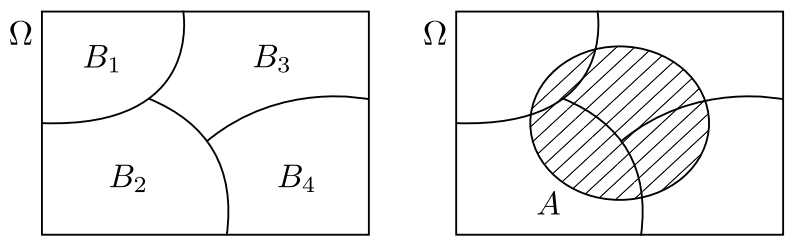
\includegraphics[width=\linewidth,keepaspectratio]{pictures/satz_der_totalen_wahrscheinlichkeit.png} 
\end{figure}

\DEF{Multiplikationsregel}{Seien $A_1,...,A_n\in\mathcal{F}$. Falls $\P[\bigcap_{i=1}^nA_i]>0$. Dann $\P[\bigcap_{i=1}^nA_i]=\P[A_1]\cdot\P[A_2|A_1]\cdot\P[A_3|A_1\cap A_2]\cdot ... \cdot\P[A_n|A_1\cap ...\cap A_{n-1}]$.}

\DEF{Satz von Bayes}{Sei $B_1, ...,B_N$ mit $\P[B_n]>0$ $\forall$ $n\in\{1,...,N\}$ eine Partition von $\Omega$. Dann $\forall$ $A\in\mathcal{F}$ mit $\P[A]>0$ gilt $\P[B_n|A]=\frac{\P[A|B_n]\P[B_n]}{\sum_{k=1}^N\P[A|B_k]\P[B_k]}$.}

\DEF{Satz von Bayes (Spezialfall $n=2$)}{$\P[B|A]=\frac{\P[A|B]\P[B]}{\P[A|B]\P[B] + \P[A|B^\complement]\P[B^\complement]}=\frac{\P[A\cap B]}{\P[A]}$.}




\mysubsection{Unabhängigkeit}
\DEF{Unabhängigkeit von 2 Ereignissen}{$A,B\in\mathcal{F}$ sind (stochastisch) unabhängig $\Leftrightarrow \P[A\cap B]=\P[A]\P[B] \Leftrightarrow \P[A|B]=\P[A] \Leftrightarrow \P[B|A]=\P[B]$.
\begin{itemize}
    \item $\P[A]\in\{0,1\} \Rightarrow \P[A\cap X]=\P[A]\P[X]$ $\forall$ $X\subseteq\mathcal{F} \Leftrightarrow A$ ist unabhängig von jedem Ereignis.
    \item $A$ ist unabhängig von sich selbst $\Leftrightarrow \P[A\cap A]=\P[A]^2 \Rightarrow \P[A]\in\{0,1\}$.
    \item $\P[A\cap B]=\P[A]\P[B] \Leftrightarrow \P[A\cap B^\complement]=\P[A]\P[B^\complement]$.
\end{itemize}}

\DEF{Unabhängigkeit von n Ereignissen}{Sei $I$ eine beliebige Indexmenge. Eine Familie von Ereignissen $(A_i)_{i\in I}$ ist (stochastisch) unabhängig $\Leftrightarrow $ $\forall$ $J\subset I$ gilt $\P[\bigcap_{j\in J}A_j]=\prod_{j\in J}\P[A_j]$.}

\DEF{Paarweise Unabhängigkeit}{Produktformel gilt nur für alle Paare von Ereignissen. Unabhängigkeit $\Rightarrow$ paarweise Unabhängigkeit $\not\Rightarrow$ Unabhängigkeit.}




\mysubsection{Zufallsvariablen}
\DEF{Zufallsvariable}{Eine (reellwertige) Zufallsvariable (ZV) ist eine Abbildung $X:\Omega\rightarrow\R$ $(\omega\mapsto X(\omega))$ s.d. $\forall$ $x\in\R$ gilt $\{\omega\in\Omega|X(\omega)\leq x\}\in\mathcal{F} \Leftrightarrow \{\omega\in\Omega|X(\omega)\in (-\infty,x]\}\in\mathcal{F} \Leftrightarrow \{\omega\in\Omega|X(\omega)\in B\}\in\mathcal{F}$ wobei $B=(-\infty,x]\in\mathcal{B}(\R) \Leftrightarrow X$ ist eine messbare Funktion.}

\DEF{Diskrete Zufallsvariable}{Eine ZV $X:\Omega\rightarrow\R$ heisst diskret, falls eine endliche oder abzählbare Menge $W\subset\R$ existiert, s.d. $\P[X\in W]=1$, wenn also die Werte von $X$ fast sicher in $W$ liegen.

Wenn $\Omega$ endlich oder abzählbar $\Rightarrow$ jede ZV $X:\Omega\rightarrow\R$ diskret.}

\DEF{Urbild}{Sei $X$ eine ZV. Sei $B\in\mathcal{B}(\R)$. Dann $X^{-1}(B):=\{\omega\in\Omega|X(\omega)\in B\}$ wobei für Messbarkeit $X^{-1}(B)\in\mathcal{F}$ $\forall B\in\mathcal{B}(\R)$ gelten muss.}

\DEF{Indikatorfunktion auf $A\in\mathcal{F}$}{
$1_A(\omega)=\begin{cases}
0 & \text{if } \omega\not\in A,\\
1 & \text{if } \omega\in A.
\end{cases}$

$\{\omega\in\Omega|1_A(\omega)\leq x\}=\begin{cases}
\emptyset & \text{if } x<0,\\
A^\complement & \text{if } 0\leq x< 1,\\
\Omega & \text{if } x\geq 1.
\end{cases}$
}

\DEF{Komposition}{Sei $X:\Omega\rightarrow\R$ eine ZV und $\phi:\R\rightarrow\R$ eine Funktion. Dann ist die Komposition $\phi(X):=\phi\circ X:\Omega\rightarrow\R$ ebenfalls eine ZV.
\begin{align*}
    \Omega \stackrel{X}{\rightarrow} \R& \stackrel{\phi}{\rightarrow}  \R\\
    \omega \mapsto X(\omega)& \mapsto  \phi(X(\omega))
\end{align*}
Für $n$ ZV $X_1,...,X_n$ und eine Abbildung $\phi:\R_n\rightarrow\R$ schreiben wir $\phi(X_1,...,X_n):=\phi\circ(X_1,...,X_n):\Omega\rightarrow\R$. Wobei $\phi$ eine Funktion mit mehreren Parametern ist.}

\DEF{Notation}{
\begin{align*}
    \{X\leq x\}&:=\{\omega\in\Omega|X(\omega)\leq x\},\\
    \{x<X\leq y\}&:=\{\omega\in\Omega|X(\omega)\in (x,y], x<y\},\\
    \{X\in\N\}&:=\{\omega\in\Omega|X(\omega)\in\N\},\\
    \hdots\\
    \P[X\leq x]&:=\P[\{X\leq x\}]=\P[\{\omega\in\Omega|X(\omega)\leq x\}],\\
    \hdots
\end{align*}}

\DEF{Unabhängigkeit}{Die ZV $X_1,...,X_n$ heissen unabhängig, wenn $\forall x_1,...,x_n\in\R$ gilt $\P[X_1\leq x_1,...,X_n\leq x_n]=\P[X_1\leq x_1]\cdot ... \cdot\P[X_n\leq x_n] \Leftrightarrow$ $\forall I_1\in\R,...,I_n\in\R$ die Ereignisse $\{X_1\in I_1\},...,\{X_n\in I_n\}$ unabhängig sind.}

\DEF{Gruppierung}{Seien $X_1,...,X_n$ unabhängige ZV. Seien $1\leq i_1 < i_2 < ... < i_k \leq n$ Indexe und $\phi_1,...\phi_k$ Abbildungen. Dann sind $Y_1:=\phi_1(X1,...,X_{i_1}),Y_2:=\phi_2(X_1,...,X_{i_2}),...,Y_k:=\phi_k(X_1,...,X_{i_k})$ unabhängig.}




\mysubsection{Verteilungsfunktion}
\DEF{Verteilungsfunktion (cumulative distribution function, cdf)}{Sei $X$ eine ZV auf $(\Omega,\mathcal{F},\P)$. Dann ist die cdf die Funktion $F_X:\R\rightarrow[0,1]$, definiert durch $x\mapsto F_X(x):=\P[X\leq x]$ und erfüllt folgende Eigenschaften:
\begin{enumerate}
    \item $F_X$ ist monoton wachsend.
    \item $F_X$ ist rechtsstetig, d.h. $\forall x\in\R$ gilt $F_X(x)=lim_{h\rightarrow 0}F_X(x+h)$.
    \item $lim_{x\rightarrow -\infty}F_X(x)=0$ und $lim_{x\rightarrow\infty}F_X(x)=1$.
\end{enumerate}}

\SA{}{Sei $X$ eine reellwertige ZV und seien $a,b\in\R$ mit $a<b$. Dann $\P[a<X\leq b]=F_X(b)-F_X(a)$.}

\DEF{Gemeinsame Verteilungsfunktion (joint cumulative distribution function, jcdf)}{Seien $X_1,...,X_n$ ZV. Dann ist die jcdf eine Abbildung $F:\R^n\rightarrow[0,1]$ definiert durch $(x_1,...,x_n)\mapsto F(x_1,...x_n)=\P[X_1\leq x_1,...,X_n\leq x_n]$.}

\DEF{Unabhängig und identisch verteilt (idependent and identically distributed, i.i.d.)}{Eine Folge von ZV $X_1,X_2,...$ heisst i.i.d. falls sie unabhängig ist und die ZV dieselbe cdf haben. d.h. $F_{X_k}=F_{X_l}$ $\forall$ $k,l\in\N$.}

\DEF{Unstetigkeit der Verteilungsfunktion}{Für $X\sim Ber(p)$ mit $p < 1$ gilt $\forall h>0$ $F_X(-h)=0$. Aber $F_X(0)=1-p\not = 0 \Leftrightarrow F$ nicht linksstetig in $0$. Also $lim_{h\rightarrow 0}F_U(-h)=0\not =F_X(0)$.}

\DEF{Linksseitiger Grenzwert im Punkt x}{$F(x-):=lim_{h\rightarrow 0}F(x-h)$.}

\DEF{Wahrscheinlichkeit eines Punktes}{Sei $X:\Omega\rightarrow\R$ eine ZV mit cdf $F$. Dann $\forall x\in\R$ gilt $\P[X=x]=F(x)-F(x-)=F(x)-lim_{h\rightarrow 0}F(x-h)$.}




\mysubsection{Konstruktion gleichverteilter ZV}
\DEF{Existenzsatz von Kolmogorov}{Es existiert ein $(\Omega,\mathcal{F},\P)$ und eine unendliche Folge von i.i.d. Bernoulli Zufallsvariablen $X_1,X_2,...$ auf $(\Omega,\mathcal{F},\P)$ mit Parameter $\frac{1}{2}$.}

\DEF{Gleichverteilt}{Sei $U$ eine ZV. $U$ ist gleichverteilt auf $[0,1]$ $\Leftrightarrow U\sim\mathcal{U}([0,1]) \Leftrightarrow F_U(x) = \begin{cases}
    0 & \text{if } x<0, \\
    x & \text{if } 0\leq x \leq 1, \\
    1 & \text{if } x > 1.
\end{cases}$}

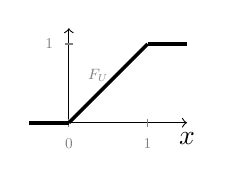
\begin{tikzpicture}
    \draw[->] (-0.5, 0) -- (1.5, 0) node[below] {$x$};
    \draw[->] (0, 0) -- (0, 1.2);
    \foreach \x in {0, 1} {
        \draw [gray] (\x, 0.05) -- ++(0, -.1) ++(0, -.15) node [below, outer sep=0pt, inner sep=0pt, scale=0.6] {\small\(\x\)};}
    \foreach \y in {1} {
        \draw [gray] (0.05, \y) -- ++(-.1, 0) ++(-.15, 0) node [left, outer sep=0pt, inner sep=0pt, scale=0.6] {\small\(\y\)};}
    \draw [gray] (0.5, 0.6) node [left, outer sep=0pt, inner sep=0pt, scale=0.6] {\small\(F_U\)};
    \draw[draw=black,line width=1.3pt] (-0.5,0) -- (0,0);
    \draw[draw=black,line width=1.3pt] (0,0) -- (1,1);
    \draw[draw=black,line width=1.3pt] (1,1) -- (1.5,1);
\end{tikzpicture}

\SA{}{Sei $X_1,X_2,...$ eine Folge unabhängiger Bernoulli-ZV mit Parameter $\frac{1}{2}$. Also $\forall \omega\in\Omega$ gilt $X_1(\omega),X_2(\omega),...\in\{0,1\}$. Somit konvergiert die Reihe $X(\omega):=\sum_{n=1}^{\infty}2^{-n}X_n(\omega)$ absolut. Weiter ist $X:\Omega\rightarrow[0,1]$ eine gleichverteilte ZV auf $[0,1]$.}

\DEF{Binärdarstellung}{Jedes $x\in[0,1)$ kann eindeutig in der Form $x=\sum_{n=1}^{\infty}2^{-n}x_n=\frac{1}{2}x_1+\frac{1}{4}x_2+\frac{1}{8}x_3+...$ dargestellt werden, wobei $x_n\in\{0,1\} \forall n\in\N$ und $\forall N\in\N \exists k>N$ s.d. $x_k=0$ (also die Folge "endet" nicht in unendlich vielen 1-en). Die Folge $\{x_n\}_{n\in\N}$ heisst Binärdarstellung von $x$ und wir schreiben $x=(.x_1x_2x_3...)_2$.}




\mysubsection{Konstruktion beliebig verteilter ZV}
\DEF{Verallgemeinerte Inverse}{Sei $F:\R\rightarrow[0,1]$ eine cdf. Dann ist die Abbildung $F^{-1}:(0,1)\rightarrow\R$ definiert durch $F^{-1}(\alpha)=inf\{x\in\R|F(x)\geq\alpha\}$ die verallgemeinerte inverse cdf von $F$.

Da $F$ rechtsstetig gilt $\forall x\in\R$ und $\alpha\in(0,1)$, dass $F^{-1}(\alpha)\leq x\Leftrightarrow \alpha\leq F(x)$.}

\DEF{Inversionsmethode}{Sei $F:\R\rightarrow [0,1]$ eine cdf. Sei $U\sim\mathcal{U}([0,1])$. Dann hat die ZV $X:=F^{-1}(U)$ die cdf $F$.}

\SA{}{Sei $F_1,F_2,...$ eine Folge von cdf. Dann $\exists (\Omega,\mathcal{F},\P)$ und eine Folge von ZV $X_1,X_2,...$ auf $(\Omega,\mathcal{F},\P)$, s.d. $\forall k\in\N$ gilt $X_k$ hat cdf $F_k$ und $X_1,X_2,...$ sind unabhängig.}



\mysubsection{Gewichtsfunktion}
\DEF{Gewichtsfunktion (diskrete dichte, probability mass function, pmf)}{Sei $X$ mit Wertebereich $W(X)=\{x_1,x_2,...\}$ und den dazugehörigen Wahrscheinlichkeiten $\{p1,p2,...\}$ eine diskrete ZV. Dann ist die pmf definiert als $p_X:W(X)\rightarrow[0,1]$ mit $p_X(x_k):=\P[X=x_k]=p_k$ und hat folgende Eigenschaften:
\begin{itemize}
    \item $\forall x_k\in W(X)$ gilt $p_X(x_k)\in[0,1]$.
    \item $\sum_{x_k\in W(X)}p_X(x_k)=\P[X\in W(X)]=1$.
\end{itemize}

Die Zahlenfolge $\{p_X(x_k)\}_{x_k\in W(X)}$ wird auch Verteilung von $X$ genannt.}

\SA{}{Sei $X$ eine diskrete ZV mit Werten in $W$ und pmf $p_X$. Dann ist die cdf von $X$ gegeben durch $F_X(x)=\P[X\leq x]=\sum_{y\in W,y\leq x}p_X(y)$. Weiter gilt für jede messbare Teilmenge $B\subseteq W$, dass $\P[X\in B]=\sum_{x\in B}p_X(x)$.}

\DEF{Gemeinsame Gewichtsfunktion}{Seien $X,Y$ diskrete ZV mit Wertebereichen $W_X$ und $W_Y$. Seien $x\in W_X,y\in W_Y$. Dann ist ihre gemeinsame pmf definiert als $p_{X,Y}: W_X\times W_Y\rightarrow[0,1]$ mit $p_{X,Y}(x,y):=\P[X=x,Y=y]$.}

\DEF{Randgewicht}{Seien $X,Y$ diskrete ZV mit Wertebereichen $W_X$ und $W_Y$. Sei $x\in W_X$. Dann ist das Randgewicht von $X$ definiert als $p_X(x)=\sum_{y\in W_Y}f_{X,Y}(x,y)$.}


\mysubsection{Diskrete Verteilungen}
\DEF{Bernoulli}{Sei $p\in[0,1]$. ZV $X$ ist Bernoulli ZV mit parameter $p \Leftrightarrow X\sim Ber(p) \Leftrightarrow$ $\forall\omega\in\Omega: X(\omega)\in\{0,1\}=W_X\ \land$\\ $\forall k\in W_X: p_X(k)=\P[X=k]=\begin{cases}
    p & \text{if $k=1$,}\\
    1-p & \text{if $k=0$.}
\end{cases}$ 

\begin{enumerate}
    \item $\E[X]=p$.
    \item $\V[X]=p(1-p)$.
\end{enumerate}}

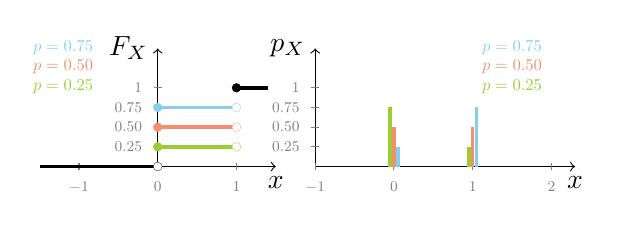
\begin{tikzpicture}
\begin{scope}
    % Axis
    \draw[->] (-1.5, 0) -- (1.5, 0) node[below]{$x$};
    \draw[->] (0, 0) -- (0, 1.5) node[left]{$F_X$};

    % Axis labels
    \foreach \x in {-1, ..., 1} {
        \draw [gray] (\x, 0.05) -- ++(0, -.1) ++(0, -.15) node [below, outer sep=0pt, inner sep=0pt, scale=0.6] {\small\(\x\)};}
    \foreach \y in {0.25, 0.50, 0.75, 1} {
        \draw [gray] (0.05, \y) -- ++(-.1, 0) ++(-.15, 0) node [left, outer sep=0pt, inner sep=0pt, scale=0.6] {\small\(\y\)};}

    % Definitions
    \def\pOne {0.25}
    \def\pTwo {0.50}
    \def\pThree {0.75}

    \def\firstColor {YellowGreen};
    \def\secondColor {Melon};
    \def\thirdColor {SkyBlue};
    
    % Legend
    \node [above, text=\firstColor,scale=0.6] at (-1.2,\pOne + 0.6) {$p = \pOne$};
    \node [above, text=\secondColor,scale=0.6] at (-1.2,\pTwo + 0.6) {$p = \pTwo$};
    \node [above, text=\thirdColor,scale=0.6] at (-1.2,\pThree + 0.6) {$p = \pThree$};
    
    % Function
    \draw[draw=black,line width=1.3pt] (-1.5,0) -- (0,0);
    \filldraw[draw=black,line width=0.1pt,fill=white] (0,0) circle[radius=1.6pt];

    \draw[draw=\firstColor,line width=1.3pt] (0,\pOne) -- (1,\pOne);
    \filldraw[draw=\firstColor,line width=0.1pt,fill=\firstColor] (0,\pOne) circle[radius=1.6pt];
    \filldraw[draw=\firstColor,line width=0.1pt,fill=white] (1,\pOne) circle[radius=1.6pt];

    \draw[draw=\secondColor,line width=1.3pt] (0,\pTwo) -- (1,\pTwo);
    \filldraw[draw=\secondColor,line width=0.1pt,fill=\secondColor] (0,\pTwo) circle[radius=1.6pt];
    \filldraw[draw=\secondColor,line width=0.1pt,fill=white] (1,\pTwo) circle[radius=1.6pt];

    \draw[draw=\thirdColor,line width=1.3pt] (0,\pThree) -- (1,\pThree);
    \filldraw[draw=\thirdColor,line width=0.1pt,fill=\thirdColor] (0,\pThree) circle[radius=1.6pt];
    \filldraw[draw=\thirdColor,line width=0.1pt,fill=white] (1,\pThree) circle[radius=1.6pt];
    
    \draw[draw=black,line width=1.3pt] (1,1) -- (1.4,1);
    \filldraw[draw=black,line width=0.1pt,fill=black] (1,1) circle[radius=1.6pt];
\end{scope}
\begin{scope}[xshift=3cm]
    % Axis
    \draw[->] (-1, 0) -- (2.3, 0) node[below]{$x$};
    \draw[->] (-1, 0) -- (-1, 1.5) node[left]{$p_X$};

    % Axis labels
    \foreach \x in {-1, ..., 2} {
        \draw [gray] (\x, 0.05) -- ++(0, -.1) ++(0, -.15) node [below, outer sep=0pt, inner sep=0pt, scale=0.6] {\small\(\x\)};}
    \foreach \y in {0.25, 0.50, 0.75, 1} {
        \draw [gray] (-0.95, \y) -- ++(-.1, 0) ++(-.15, 0) node [left, outer sep=0pt, inner sep=0pt, scale=0.6] {\small\(\y\)};}

    % Definitions
    \def\pOne {0.25}
    \def\pTwo {0.50}
    \def\pThree {0.75}

    \def\firstColor {YellowGreen};
    \def\secondColor {Melon};
    \def\thirdColor {SkyBlue};
    
    % Legend
    \node [above, text=\firstColor,scale=0.6] at (1.5,\pOne + 0.6) {$p = \pOne$};
    \node [above, text=\secondColor,scale=0.6] at (1.5,\pTwo + 0.6) {$p = \pTwo$};
    \node [above, text=\thirdColor,scale=0.6] at (1.5,\pThree + 0.6) {$p = \pThree$};
    
    % Function
    \draw[draw=\firstColor,line width=1.3pt] (-0.05,0) -- (-0.05,1-\pOne);
    \draw[draw=\secondColor,line width=1.3pt] (0,0) -- (0,1-\pTwo);
    \draw[draw=\thirdColor,line width=1.3pt] (0.05,0) -- (0.05,1-\pThree);    

    \draw[draw=\firstColor,line width=1.3pt] (0.95,0) -- (0.95,\pOne);    
    \draw[draw=\secondColor,line width=1.3pt] (1,0) -- (1,\pTwo);
    \draw[draw=\thirdColor,line width=1.3pt] (1.05,0) -- (1.05,\pThree);
\end{scope}
\end{tikzpicture}
\DEF{Binomialverteilung}{Modelliert die Anzahl Erfolge bei wiederholten Bernoulli-Experimenten. Sei $p\in[0,1]$ und $n\in\N$. ZV $X$ ist binomialverteilt mit Parametern $n$ und $p$ $\Leftrightarrow$ $X\sim Bin(n,p) \Leftrightarrow$ $\forall\omega\in\Omega: X(\omega)\in\{0,...,n\}=W_X\ \land\ \forall k\in W_X:p_X(k)=\P[X=k]={n\choose k} p^k(1-p)^{n-k}$.

\begin{enumerate}
    \item $\E[X]=np$.
    \item $\V[X]=np(1-p)$.
\end{enumerate}}

\SA{}{Sei $p\in[0,1]$ und $n\in\N$. Seien $X_1,...,X_n\sim Ber(p)$ alle unabhängig. Dann gilt $S_n:=X_1+...+X_n\sim Bin(n,p)$.}

\DEF{Geometrische Verteilung}{Sei $p\in(0,1]$. ZV $X$ ist geometrisch verteilt mit Parameter $p \Leftrightarrow X\sim Geom(p) \Leftrightarrow \forall\omega\in\Omega: X(\omega)\in\N=W_X\ \land\ \forall k\in W_X:p_X(k)=\P[X=k]=p(1-p)^{k-1}$. Für den Fall $p=1$ und $k=1$ erhalten wir einen Term $0^0$. Wir verwenden die Konvention $0^0=1$ und damit gilt $\P[X=1]=p$. 

\begin{enumerate}
    \item $F_X(x)=1-(1-p)^{x}$.
    \item $\E[X]=\frac{1}{p}$.
    \item $\V[X]=\frac{1-p}{p^2}$.
    \item Intuition: Modelliert die Wartezeit bis zum ersten Erfolg in einer unendlichen Folge von Bernoulli-Experimenten.
    \item Gedächtnislosigkeit: $\forall n \geq 0$ und $\forall k\geq 1$ gilt $\P[T\geq n+k|T>n]=\P[T\geq k]$.
\end{enumerate}}

\SA{}{Sei $X_1,X_2,...$ eine unendliche Folge von unabhängigen Bernoulli-Zufallsvariablen mit Parameter $p$. Dann ist $T:=inf\{n\geq 1|X_n=1\} \Rightarrow T\sim Geom(p)$.}

\DEF{Negativbinomiale Verteilung}{Verallgemeinerung der geom. Verteilung. Modelliert die Wartezeit bis zum $r$-ten Erfolg in einer unendlichen Folge von Ber.-Experimenten. ZV $X$ ist negativbinomial verteilt mit $r\in\N$ und $p\in[0,1] \Leftrightarrow X\sim NBin(r,p) \Leftrightarrow$ $\forall\omega\in\Omega: X(\omega)\in\{r,r+1,r+2,...\}=W_X\ \land\ \forall k\in W_X:p_X(k)=\P[X=k]={{k-1}\choose{r-1}}p^r(1-p)^{k-r}$. 

\begin{enumerate}
    \item $\E[X]=$.
    \item $\V[X]=$.
\end{enumerate}}

\SA{}{Sei $X_1,X_2,...$ eine unendliche Folge von unabhängigen Bernoulli-Zufallsvariablen mit Parameter $p$. Dann ist $T_r:=inf\{n\geq 1|\sum_{l=1}^nX_l=r\} \Rightarrow T_r\sim NBin(r,p)$.}

\SA{}{Seien $X_1,...,X_r\sim Geom(p)$ und unabhängige ZV. Dann ist ihre Summe $X=X_1+...+X_r\sim NBin(r,p)$.}

\DEF{Hypergeometrische Verteilung}{Seien in einer Urne $n$ Gegenstände, davon $r$ vom Typ 1 und $n-r$ vom Typ 2. Man ziehe $m$ Gegenstände ohne Zurücklegen. Dann ist ZV $X\sim H(n,r,m)$ die \# gezogener Gegenstände $k$ vom Typ 1. ZV $X$ ist hypergeometrisch verteilt mit Parametern $n\in\N$, $m,r\in\{1,...,n\} \Leftrightarrow X\sim H(n,r,m) \Leftrightarrow$ $\forall k\in\{0,1,...,min(m,r)\}$ gilt $\P[X=k]=\frac{{r\choose k}{n-r\choose m-k}}{{n\choose m}}$.

\begin{enumerate}
    \item $\E[X]=$.
    \item $\V[X]=$.
\end{enumerate}}

\DEF{Poisson-Verteilung}{Grenzwert der Binomial-Verteilung. Sei $\lambda\in\R,\lambda>0$. ZV $X$ ist Poisson-verteilt mit Parameter $\lambda \Leftrightarrow X\sim Poisson(\lambda) \Leftrightarrow \forall\omega\in\Omega:X(\omega)\in\N_0=W_X\ \land\ \forall k\in\N_0:p_X(k)=\P[X=k]=\frac{\lambda^k}{k!}e^{-\lambda}=\frac{e^{-\lambda}\lambda^k}{k!}$.

\begin{enumerate}
    \item $\E[X]=\V[X]=\lambda$.
\end{enumerate}}

\SA{}{Sei $\lambda > 0$. $\forall n\geq 1$ betrachten wir $n$ ZV $X_n\sim Bin(n,\lambda)$. Sei $N\sim Poisson(\lambda)$. Dann gilt $\forall k\in\N$, $lim_{n\rightarrow\infty}\P[X_n=k]=\P[N=k]$.}

\SA{}{Seien $X,Y$ reellwertige unabhängige ZV. Seien $\lambda,\mu>0$. Wenn $X\sim\mathcal{P}(\lambda), Y\sim\mathcal{P}(\mu)$ $\Rightarrow$ $X+Y\sim\mathcal{P}(\lambda+\mu)$.}



\mysubsection{Stetige Verteilungen}
\DEF{Stetig verteilte Zufallsvariable und Dichtefunktion (probability density function, pdf)}{ZV $X$ heisst stetig $\Leftrightarrow \exists f_X:\R\rightarrow\R_+:F_X(x)=\int_{-\infty}^xf_X(t)dt$. Wir nennen $f_X$ die pdf von $X$. Intuition: $f_X(t)dt$ ist die Wahrscheinlichkeit, dass $X\in[t,t+dt]$.}

\DEF{Stückweise stetig differenzierbare Funktionen}{Funktion $f$ ist stückweise stetig differenzierbar $\Leftrightarrow\ \exists$ eine Partition $-\infty = x_0 < x_1 < ... < x_{n-1} < x_n = \infty$ s.d. $f$ auf jedem Intervall $(x_i,x_{i+1})$ stetig differenzierbar ist.}

\SA{3.39.}{Sei $X$ eine ZV. Sei $F_X$ stetig und stückweise stetig differenzierbar auf einer Partition $-\infty=x_0<x_1<...<x_{n-1}<x_n=\infty \Rightarrow X$ ist eine stetige ZV und $f_X=\begin{cases}
    F_X'(x) & \text{if $\exists k\in\{0,...,n-1\}:x\in(x_k,x_{k+1}),$}\\
    a_k & \text{if $x\in\{x_1,...,x_{n-1}\},$}
\end{cases}$ wobei $a_k$ beliebig gewählt werden dürfen. Es gilt also $f_X(x)=F_X'(x)$ in allen Stetigkeitspunkten $x$ von $f_X$.}

\NOTE{$f_X$ vs. $p_X$}{Die pdf $f_X$ ist (fast exakt) das stetige Analogon zur pmf $p_X$ einer diskreten ZV.

\begin{enumerate}
    \item Für messbare Mengen $B\subset\R$ gilt $\P[X\in B]=\int_Bf_X(x)dx$ analog zu $\P[X\in B]=\sum_{x\in B}p_X(x)$.
    \item Da allerdings $\P[X=x]=0\ \forall x\in\R$, hat in diesem Sinn $X$ keine pmf wie diskrete ZV.
    \item Ist $f_X$ allerdings stetig an der Stelle $x$, so haben wir $f_X(x)=lim_{\varepsilon\rightarrow 0}\frac{1}{\varepsilon}\int_x^{x+\varepsilon}f_X(t)dt=lim_{\varepsilon\rightarrow0}\frac{\P[x<X\leq x+\varepsilon]}{\varepsilon}$ und somit $\P[X\in(x,x+\varepsilon)]\approx\varepsilon f_X(x)$ für kleine $\varepsilon$. Dies wird oft auch als $\P[X\in(x,x+dx]]=f_X(x)dx$ geschriben.
    \item Nach Satz 3.39 gilt für stetige Dichten, dass Verteilungsfunktion und Dichte auseinander durch Integrieren bzw. Differenzieren entstehen.
    \item Merkregel: Vom diskreten zum stetigen Fall kommt man, indem man die Kombination (Summe, Gewichtsfunktion bzw. pmf) systematisch durch (Integral, Dichtefunktion bzw. pdf) ersetzt.
\end{enumerate}}

\DEF{Gleichverteilung}{ZV $X$ ist gleichverteilt auf $[a,b] \Leftrightarrow X\sim\mathcal{U}([a,b]) \Leftrightarrow f_X(x)=\begin{cases}
    \frac{1}{b-a} & \text{$x\in[a,b],$}\\
    0 & \text{sonst.}
\end{cases}$

\begin{figure}[H]
 \centering
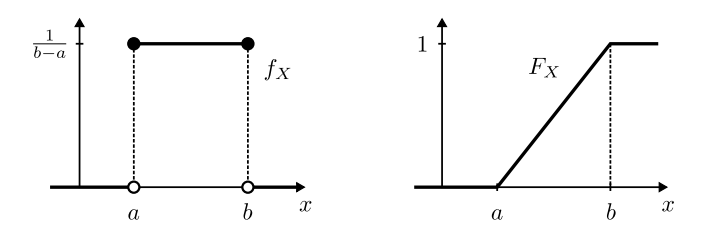
\includegraphics[width=\linewidth,keepaspectratio]{pictures/uniform_distribution.png} 
\end{figure}

\begin{enumerate}
    \item $\E[X]=\frac{a+b}{2}$.
    \item $\V[X]=\frac{(b-a)^2}{12}$.
    \item Intuition: Modelliert die zufällige Wahl eines Punktes in $[a,b]$.
\end{enumerate}}

\DEF{Exponentialverteilung}{ZV $X$ ist exponentialverteilt mit $\lambda > 0 \Leftrightarrow X\sim Exp(\lambda) \Leftrightarrow$ $\forall x\in\R:f_X(x)=\begin{cases}
    \lambda e^{-\lambda x} & \text{$x\geq 0,$}\\
    0 & \text{$x<0.$}
\end{cases}$

\begin{figure}[H]
 \centering
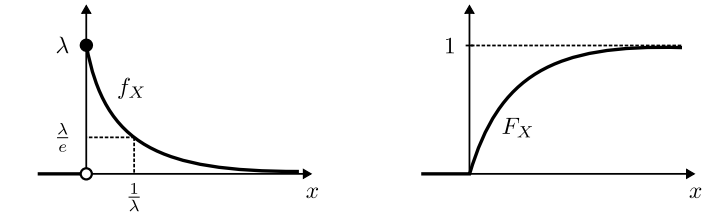
\includegraphics[width=\linewidth,keepaspectratio]{pictures/exponential_distribution.png} 
\end{figure}

\begin{enumerate}
    \item $F_X(x)=1-e^{-\lambda x}\Leftrightarrow F_X^{-1}(y)=\frac{-1}{\lambda}log(1-y)$.
    \item $\E[X]=\frac{1}{\lambda}$.
    \item $\V[X]=\frac{1}{\lambda^2}$.
    \item Intuition: Ist das stetige Analogon der geometrischen Verteilung. Modelliert die Wartezeit oder Lebensdauer für beliebige Werte $x\geq 0$.
    \item Besitzt auch die Eigenschaft der Gefächtnislosigkeit, also $\P[X>t+s|X>s]=\P[X>t]$.
\end{enumerate}}

\DEF{Cauchy-Verteilung}{ZV $X$ ist Cauchy-verteilt mit $x_0\in\R,\gamma > 0 \Leftrightarrow X\sim Cauchy(x_0,\gamma) \Leftrightarrow$ $f_X(x)=\frac{1}{\pi}\frac{\gamma}{\gamma^2+(x-x_0)^2}$.
\begin{figure}[H]
 \centering
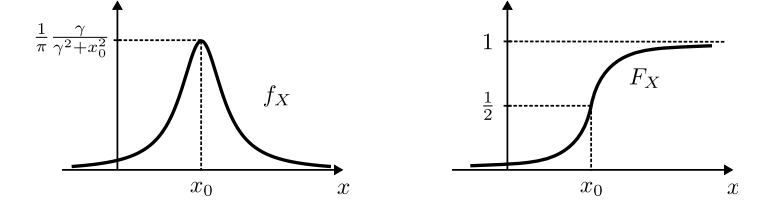
\includegraphics[width=\linewidth,keepaspectratio]{pictures/cauchy_distribution.png} 
\end{figure}

\begin{enumerate}
    \item $F_X(x)=\frac{1}{2}+\frac{1}{\pi}\arctan(x)\Leftrightarrow F_X^{-1}(y)=\tan((y-\frac{1}{2})\pi)$.
    \item $\E[X]$ undefiniert, $\E[X_+]=\E[X_-]=\infty$.
    \item Weiter gilt $F_X(x)=\frac{1}{2}+\frac{1}{\pi}arctan(\frac{x-x_0}{\gamma})$.
    \item $Y,Z$ unabhängige $\mathcal{N}(0,1)$-verteilte ZV $\Rightarrow \frac{Y}{Z}=X\sim Cauchy(0,1)$.
    \item Ist eine langschwänzige Verteilung (heavytailed distribution). $f_X(x)$ geht für $|x|\rightarrow\infty$ nur sehr langsam gegen 0 (quadratisch, im Vergelich zum exponentiellen Abfallen bei der Normalverteilung).
\end{enumerate}}

\DEF{Normalverteilung}{ZV $X$ ist normalverteilt mit $\mu\in\R,\sigma^2>0 \Leftrightarrow X\sim\mathcal{N}(\mu,\sigma^2) \Leftrightarrow$ $f_X(x)=\frac{1}{\sigma\sqrt{2\pi}}e^{-\frac{1}{2}(\frac{x-\mu}{\sigma})^2}$.
\begin{figure}[H]
 \centering
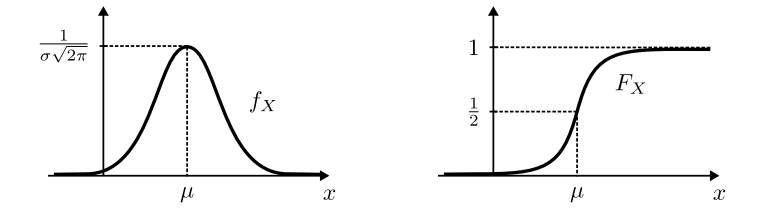
\includegraphics[width=\linewidth,keepaspectratio]{pictures/normal_distribution.png} 
\end{figure}

\begin{enumerate}
    \item $\E[X]=\mu$.
    \item $\V[X]=\sigma^2$.
    \item Wird auch als gausssche Glockenkurve, Gauss-Funktion, gausssche Normalverteilung, gausssche Verteilungskurve, Gauss-Kurve, und Gauss-Glocke bezeichnet.
    \item $f_X=\varphi$ und $F_X=\Phi$. Die zugehörigen Variablen nennen wir $Z$.
    \item Weder für $F_X$ noch für $\Phi$ gibt es einen geschlossenen Ausdruck, aber das Integral $\Phi(x)=\int_{-\infty}^x\varphi(t)dt=\frac{1}{\sqrt{2\pi}}\int_{-\infty}^xe^{-\frac{t^2}{2}}dt$ ist tabelliert.
    \item Uneigentliches Integral über Normalverteilung (L4.21): $\int_{-\infty}^{\infty}e^{\frac{-x^2}{2\sigma^2}}dx=\sqrt{2\pi\sigma^2}$.
\end{enumerate}}

\DEF{Standardnormalverteilung}{Wichtiger Spezialfall der Normalverteilung mit $\mu=0, \sigma^2=1$ also $\mathcal{N}(0,1)$. Für $X\sim\mathcal{N}(\mu,\sigma^2)$ gilt $\frac{X-\mu}{\sigma}\sim\mathcal{N}(0,1),$ also $F_X(x)=\P[X\leq x]=\P[\frac{X-\mu}{\sigma}\leq\frac{x-\mu}{\sigma}]=\Phi(\frac{x-\mu}{\sigma})$. Daraus folgt, dass für $\mu\in\R,\sigma^2>0,Z\sim\mathcal{N}(0,1)$ gilt $\mu+\sigma Z\sim\mathcal{N}(\mu,\sigma^2)$.

Es gilt $\E[X^{2k}]=(2k-1)!!$, wobei $(2k-1)!!$ die Doppelfakultät ist, also das Produkt aller ungeraden Zahlen.

Um jede beliebig normalverteilte ZV $X\sim\mathcal{N}(\mu,\sigma^2)$ zu simulieren, reicht es $Z\sim\mathcal{N}(0,1)$ zu simulieren und die erhaltetnen Werte mit $\sigma$ zu multiplizieren und mit $\mu$ zu addieren.}

\SA{3.50.}{Seien $X_1,...,X_n$ unabhängige ZV s.d. $X_1\sim\mathcal{N}(\mu_1,\sigma_1^2),...,X_n\sim\mathcal{N}(\mu_n,\sigma_n^2)$. Dann $Z:=\mu_0+\sum_{k=1}^na_kX_k\sim\mathcal{N}(\mu_0+\sum_{k=1}^na_k\mu_k,\sum_{k=1}^na_k^2\sigma_k^2)$.}

\SA{3.52.}{Für $X\sim\mathcal{N}(\mu,\sigma^2)$ liegt der "Grossteil" des Wahrscheinlichkeitsmasses im Intervall $[\mu-3\sigma,\mu+3\sigma]$. Es gilt $\P[|X-\mu|\geq 3\sigma]\leq 0.0027$.}

\mysection[JungleGreen]{\centering Erwartungswert, Varianz, Covarianz}
\mysubsection{Allgemeiner Erwartungswert}
\DEF{Erwartungswert (nicht-negativ)}{Sei $X:\Omega\rightarrow\mathbb{R}_+$ eine ZV mit nicht-negativen Werten. Dann $\mathbb{E}[X]=\int_0^{\infty}(1-F_X(x))dx$ der Erwartungswert von $X$.}

\SA{}{Sei $X$ eine nicht-negative ZV. Dann gilt $\mathbb{E}[X]\geq 0$. Gleichheit gilt genau dann wenn $X=0$ fast sicher gilt.}

\DEF{Zerlegung von $X$ in positiven und negativen Teil}{ Der positive und negative Teil von $X$ sind die ZV $X_+,X_-$ definiert durch $X_+(w)=max(X,0)=\begin{cases}
    X(w) & \text{$X(w)\geq 0,$}\\
    0 & \text{$X(w)<0,$}
\end{cases}$ und $X_-(w)=-min(X,0)=max(-X,0)=\begin{cases}
    -X(w) & \text{$X(w)\leq 0,$}\\
    0 & \text{$X(w)>0.$}
\end{cases}$. 

Es gilt $X=X_+-X_-$ und $|X|=X_++X_-$.}

\DEF{Allgemeiner Erwartungswert}{Sei $X$ eine reellwertige ZV. $\mathbb{E}[|X|]<\infty \Rightarrow \mathbb{E}[X_-],\mathbb{E}[X_+]<\infty \Rightarrow \mathbb{E}[X]=\mathbb{E}[X_+]-\mathbb[X_-]$. 

Für $X\geq 0$ ist $\mathbb{E}[X]$ immer definiert und kann endlich oder unendlich sein. Wenn $X$ hingegen kein konstantes Vorzeichen hat und $\mathbb{E}[|X|]<\infty$ nicht erfüllt $\Rightarrow \mathbb{E}[X]$ undefiniert.}


\mysubsection{Erwartungswert diskreter ZV}
\DEF{Erwartungswert (diskret)}{Sei $X:\Omega\rightarrow\mathbb{R}$ eine diskrete ZV, deren Werte fast sicher in $W$ (endlich oder abzählbar) liegen. Dann gilt $\mathbb{E}[X]=\sum_{x\in W}x\cdot\mathbb{P}[X=x]=\sum_{x\in W}x\cdot p_X(x)$, sofern $\mathbb{E}[X]$ wohldefiniert.}

\SA{}{Sei $X:\Omega\rightarrow\mathbb{R}$ eine diskrete ZV. $\mathbb{E}[X]$ wohldefiniert $\Leftrightarrow$ Reihe $\sum_{x\in W}x\cdot\mathbb{P}[X=x]$ konvergiert absolut $\Leftrightarrow \sum_{x\in W}|x|\cdot\mathbb{P}[X=x]<\infty$.}

\SA{}{Sei $X:\Omega\rightarrow\mathbb{R}$ eine diskrete ZV. Sei $\varphi:\mathbb{R}\rightarrow\mathbb{R}$. Dann $\mathbb{E}[\varphi(X)]=\sum_{x\in W}\varphi(x)\cdot\mathbb{P}[X=x]$, sofern $\mathbb{E}[X]$ wohldefiniert.}


\mysubsection{Erwartungswert stetiger ZV}
\mysection[BrickRed]{Gemeinsame Verteilungen}

\mysubsection{Gemeinsame Diskrete Verteilung}
\DEF{Gemeinsame Diskrete Verteilung}{Seien $X_1,...,X_n$ diskrete ZV. Seien $W_k\subset\R$ endlich oder abzählbar s.d. $X_k\in W_k$ f.s. für $k\in[n]$.

Die gemeinsame Verteilung von $(X_1,...,X_n)$ (joint probability distribution, jpd) ist eine Familie von Wahrscheinlichkeiten $\{p(x_1,...,x_n)\}_{x_1\in W_1,...,x_n\in W_n}$, wobei $p:\R^n\rightarrow[0,1]$ die gemeinsame Gewichtsfunktion (joint probability mass function, jpmf) bezeichnet, $p(x_1,...,x_n)=\P[X_1=x_1,...,X_n=x_n]$.}

\SA{5.3}{Eine gemeinsame Verteilung von ZV $X_1,...,X_n$ erfüllt stets $$\sum_{x_1\in W_1,...,x_n\in W_n}p(x_1,...,x_n)=1.$$}

\SA{5.5}{Aus der jpmf $p$ bekommt man die jpdf $F$ via
\begin{align*}
    F(x_1,...,x_n)&=\P[X_1\leq x_1,...,X_n\leq x_n]\\
    &=\sum_{y_1\leq x_1,...,y_n\leq x_n}\P[X_1=y_1,...,X_n=y_n]\\
    &=\sum_{y_1\leq x_1,...,y_n\leq x_n}p(y_1,...,y_n).
\end{align*}}

\SA{5.6 Verteilung des Bildes}{Sei $n\geq 1$. Sei $\varphi:\R^n\rightarrow\R$. Seien $X_1,...,X_n$ diskrete ZV mit Werten jeweils in $W_1,...,W_n$ f.s. Dann ist $Z=\varphi(X_1,...,X_n)$ eine diskrete ZV, die f.s. Werte in $W=\varphi(W_1 \times ...\times W_n)$ annimmt. Zudem ist die Verteilung von $Z$ $\forall z\in W$ gegeben durch $$\P[Z=z]=\sum_{\substack{x_1\in W_1,...,x_n\in W_n,\\\varphi(x_1,...,x_n)=z}}\P[X_1=x_1,...,X_n=x_n].$$}

\SA{5.7 Randverteilung}{Seien $X_1,...,X_n$ diskrete ZV mit jpmf $p$. $\forall k\in[n]$, $\forall x\in W_k$ gilt $$\P[X_k=x]=\sum_{\substack{x_l\in W_l,\\l\in[n]\setminus\{k\}}}p(x_1,...,x_{k-1},x,x_{k+1},...,x_n).$$

Wir bezeichnen die Verteilung von $X_k$ als $k-$te Randverteilung.

Analog ist die Verteilungsfunktion der $k-$ten Randverteilung $F_{X_k}$ gegeben durch \begin{align*}
    F_{X_k}(x)&=\P[X_k\leq x]\\
&=\P[X_1<\infty,...,X_{k-1}<\infty,X_k\leq x,\\&\hspace{17px}X_{k+1}<\infty,...,X_n<\infty]\\
&=\lim_{\substack{x_l\rightarrow\infty,\\l\in[n]\setminus\{k\}}}F(x_1,...,x_{k-1},x,x_{k+1},...,x_n).
\end{align*}}

\SA{5.9 Erwartungswert des Bildes}{Seien $X_1,...,X_n$ diskrete ZV mit gemeinsamer Verteilung $\{p(x_1,...,x_n)\}_{x_1\in W_1,...,x_n\in W_n}$. Sei $\varphi:\R^n\rightarrow\R$. Dann $$\E[\varphi(X_1,...,X_n)]=\sum_{x_1,...,x_n}\varphi(x_1,...,x_n)p(x_1,...,x_n),$$ solange die Summe wohldefiniert ist, wobei wir hier über alle $x_1\in W_1,...,x_n\in W_n$ summieren.}

\SA{5.10 Unabhängigkeit}{Seien $X_1,...,X_n$ diskrete ZV mit gemeinsamer Verteilung $\{p(x_1,...,x_n)\}_{x_1\in W_1,...,x_n\in W_n}$. Äquivalent
\begin{enumerate}
    \item $X_1,...,X_n$ unabhängig
    \item $\forall x_1\in W_1,...,x_n\in W_n:$ $p(x_1,...,x_n)= \P[X_1=x_1]\cdot...\cdot\P[X_n=x_n].$
\end{enumerate}}

\mysubsection{Gemeinsame Stetige Verteilung}
\DEF{Gemeinsame stetige Verteilung}{Sei $n\geq 1$. Die ZV $X_1,...,X_n:\Omega\rightarrow\R$ besitzen eine stetige gemeinesame Verteilung, falls $\exists$ $f:\R^n\rightarrow\R_+$ s.d. $\forall a_1,...,a_n\in\R$ gilt $$\P[X_1\leq a_1,...,X_n\leq a_n]=$$ $$\int_{-\infty}^{a_1}\hdots\int_{-\infty}^{a_n}f(x_1,...,x_n)dx_n\hdots dx_1.$$

Die Funktion $f$ heisst gemeinsame Dichte von $(X_1,...,X_n)$ (joint probability density function, jpdf).}

\SA{5.12}{Sei $f$ die gemeinsame Dichte der ZV $(X_1,...,X_n)$. Dann $$\int_{-\infty}^{\infty}\hdots\int_{-\infty}^{\infty}f(x_1,...,x_n)dx_n\hdots dx_1=1.$$

Umgekehrt kann jeder Funktion $f:\R^n\rightarrow\R_+$, die obige Gleichung erfüllt, ein Wahr'raum $(\Omega,\mathcal{F},\P)$ und $n$ ZV $X_1,...,X_n$ zugeordnet werden, s.d. $f$ die gemeinsame Dichte von $X_1,...,X_n$ ist.}

\DEF{Interpretation}{Betrachen wir z.B. zwei Zufallsvariablen $X,Y$. Intuitiv beschreibt $f(x,y)dxdy$ dabei die Wahr'keit, dass ein Zuallspunkt $(X,Y)$ in einem Rechteck $[x,x+dx]\times[y,y+dy]$ liegt.}

\SA{5.15 Erwartungswert des Bildes}{Sei $\varphi:\R^n\rightarrow\R$. Falls $X_1,...,X_n$ eine gemeinsame Dichte $f$ besitzen, dann lässt sich der Erwartungswert der ZV $\varphi(X_1,...,X_n)$ berechnen als $$\E[\varphi(X_1,...,X_n)]=$$ $$\int_{-\infty}^{\infty}\hdots\int_{-\infty}^{\infty}\varphi(x_1,...,x_n)f(x_1,...,x_n)dx_n\hdots dx_1.$$}

\DEF{5.18 Randverteilung: Verteilungsfunktion}{Haben $X$ und $Y$ die gemeinsame Verteilungsfunktion $F$, so ist die Funktion $F_X:\R\rightarrow[0,1]$ gegeben durch \begin{align*}
    x\mapsto F_X(x)=\P[X\leq x]&=\P[X\leq x,Y<\infty]\\&=\lim_{y\rightarrow\infty}F(x,y)
\end{align*} die Verteilungsfunktion der Randverteilung von $X$. 

Analog ist $F_Y:\R\rightarrow[0,1]$ gegeben durch \begin{align*}
    y\mapsto F_Y(y)=\P[Y\leq y]&=\P[X<\infty,Y\leq Y]\\&=\lim_{x\rightarrow\infty}F(x,y).
\end{align*}}

\DEF{5.18 Randverteilung: Dichtefunktion}{Haben $X,Y$ eine gemeinsame Dichte $f(x,y)$, so haben auch die Randverteilungen von $X,Y$ Dichten $f_X:\R\rightarrow\R_+$ bzw. $f_Y:\R\rightarrow\R_+$. Es gilt
\begin{align*}
    f_X(x)&=\int_{-\infty}^{\infty}f(x,y)dy,\\
    f_Y(y)&=\int_{-\infty}^{\infty}f(x,y)dx.
\end{align*}}

\SA{5.21 Unabhängigkeit stetiger ZV}{Seien $X_1,...,X_n$ ZV mit Dichten $f_{X_1},...,f_{X_n}$. Äquivalent:
\begin{enumerate}
    \item $X_1,...,X_n$ unabhängig,
    \item $X_1,...,X_n$ sind gemeinsam stetig mit gemeinsamer Dichte $f:\R^n\rightarrow\R_+$, $f(x_1,...,x_n)=f_{X_1}(x_1)\cdot...\cdot f_{X_n}(x_n)$.
\end{enumerate}}





\input{sections/grenzwertsätze.tex}
\mysection[Salmon]{Statistik}

\mysubsection{Statistische Grundideen}

\DEF{Deskriptive Statistik}{Graphische Aufbereitung der Daten.}

\DEF{Induktive Statistik}{\begin{enumerate}
    \item Wir erhalten Daten $x_1,...,x_n$ und fassen diese als Realisierungen $X_1(\omega),...,X_n(\omega)$ von ZV $X_1,...,X_n$ auf.
    \item Unter geeigneten Zusatzannahmen suchen wir nach Aussagen über die Verteilung von $X_1,...,X_n$.
\end{enumerate}}

\DEF{Terminologie}{Die Gesamtheit der Beobachtungen $x_1,...,x_n$ oder Zufallsvariablen $X_1,...,X_n$ nennt man oft eine Stichprobe. Die Anzahl $n$ heisst dann der Stichprobenumfang.}

\DEF{Parameterraum}{Ausgangspunkt ist ein Datensatz $x_1,...,x_n$ aus einer Stichprobe $X_1,...,X_n$ für die wir ein Modell suchen.

\begin{enumerate}
    \item Das Modell ist beschreibbar duch einen (mögl'weise hochdimensionalen) Parameter $\vartheta$ aus dem Parameterraum $\Theta$.
    \item Wir betrachten simultan eine ganze Familie von Wahr'räumen $(\Omega,\mathcal{F},\P_{\vartheta})_{\vartheta\in\Theta}$. \begin{enumerate}
        \item Man hat typisch einen festen Grundraum $(\Omega,\mathcal{F})$, und
        \item ein $\P_{\vartheta}$ auf $(\Omega,\mathcal{F})\ \forall\ \vartheta\in\Theta$.
    \end{enumerate}
    \item Das finden von $\vartheta$ und ein passendes Modell für gegebene Daten, nennt man parametrische statistische Analyse. 
\end{enumerate}}

\DEF{Parametrische Statistische Analyse}{
\begin{enumerate}
    \item \textbf{Deskriptive Statistik:} Mit graphischen Methoden eine erste Idee für die Wahl ener geeigneten Modellierung zu finden.
    \item \textbf{Wahl eines (parametrischen) Modells:} Spezifizieren der Parametermenge und der Familie $(\P_{\vartheta})_{\vartheta\in\Theta}$ von Modellen, mit denen man arbeiten will.
    \item \textbf{Schätzung der Parameter:} Möglichst gut passendes Modell unter Benutzung eines Schätzers wählen. Die zugehörige Schätzfunktion ist eine Abbildung, die gegebenen Daten $x_1,...,x_n$ ein $\vartheta\in\Theta$ zuordnet.
    \item \textbf{Kritische Modellüberprüfung (Anpassungstest):} Überprüfen, wie gut der Parameter $\vartheta$ bzw. das Modell $\P_{\vartheta}$ zu den Daten passen, unter Verwendung statistischer Tests.
    \item \textbf{Assagen über Zuverlässigkeit der Schätzungen:} Man kann auch versuchen, einen Bereich in $\Theta$ so zu spezifizieren, dass alle zughörigen Modelle $\P_{\varepsilon}$ in einem zu präzisierenden Sinn gut zu den Daten passen. Man spricht dann avon einen Konfidenzbereich. 
\end{enumerate}}


\mysubsection{Schätzer}

\DEF{Schätzer}{Eine ZV der Form $T_l=t_l(X_1,...,X_n)$. Die Schätzfunktionen $t_l:\R^n\rightarrow\R$ müssen noch gewählt werden.

Einsetzen von Daten $x_k=X_k(\omega),k=1,...,n,$ liefert dann Schätzwerte (sample estimates) $T_l(\omega)=t_l(x_1,...,x_n)$ für $\vartheta_l,l=1,...,m$.

Der kürze halber schreiben wir oft $T=(T_1,...,T_m)$ und $\vartheta=(\vartheta_1,...,\vartheta_m)$.}

\DEF{Erwartungstreue}{Ein Schätzer $T$ heisst erwartungstreu (unbiased) für $\vartheta$, falls $\forall\vartheta\in\Theta:\E_{\vartheta}[T]=\vartheta$.

Interpretation: Im Mittel (über alle denkbaren Realisierungen $\omega$) schätzt $T$ also richtig, und zwar unabhängig davon, welches Modell $\P_{\vartheta}$ zu Grunde liegt.}

\DEF{Bias und MSE}{Sei $\vartheta\in\Theta$ und $T$ ein Schätzer.
\begin{enumerate}
    \item Der Bias (erwartete Schätzfehler) von $T$ im Modell $\P_{\vartheta}$ ist definiert als $\E_{\vartheta}[T]-\vartheta$.
    \item MSE von $T$ im Modell $\P_{\vartheta}$ ist definiert als $MSE_{\vartheta}[T]=\E_{\vartheta}[(T-\vartheta)^2]$.
    \item Eine Folge von Schätzern $T^{(n)},n\in\N$, heisst konsistent für $\vartheta$, falls $T^{(n)}$ für $n\rightarrow\infty$ in $\P_{\vartheta}-$Wahr' gegen $\vartheta$ konvergiert $\Leftrightarrow$ $\forall\vartheta\in\Theta,\forall\varepsilon >0:\lim_{n\rightarrow\infty}\P_{\vartheta}[|T^{(n)}-\vartheta|>\varepsilon]=0$.
\end{enumerate}}

\NOTE{7.7}{$MSE_{\vartheta}[T]=\E_{\vartheta}[(T-\vartheta)^2]=\V_{\vartheta}[T]+(\E_{\vartheta}[T]-\vartheta)^2$ $\Rightarrow$ $T$ erwartungstreu $\Leftrightarrow$ $MSE_{\vartheta}[T]=\V_{\vartheta}[T]$.}


\mysubsection{Maximum-Likelihood-Methode}

\DEF{Notation}{In jedem Modell $\P_{\vartheta}$ sind $(X_1,...,X_n)$ entweder
\begin{enumerate}
    \item diskret mit gemeinsamer Gewichtsfunktion $p_{\substack{\rightarrow\\ X}}(x_1,...,x_n;\vartheta)$, oder
    \item stetig mit gemeinsamer Dichtefunktion $f_{\substack{\rightarrow\\ X}}(x_1,...,x_n;\vartheta)$.
\end{enumerate}

Meistens sind die $X_k$ unter $\P_{\vartheta}$ sogar i.i.d. mit individueller $p_X(x;\vartheta)$ bzw. $f_X(x;\vartheta)$. Somit gilt
\begin{enumerate}
    \item $p_{\substack{\rightarrow\\ X}}(x_1,...,x_n;\vartheta)=\prod_{k=1}^np_X(x_k;\vartheta)$,
    \item $f_{\substack{\rightarrow\\ X}}(x_1,...,x_n;\vartheta)=\prod_{k=1}^nf_X(x_k;\vartheta)$.
\end{enumerate}

Weiter gilt $p_{\substack{\rightarrow\\ X}}(x_1,...,x_n;\vartheta)=\P_{\vartheta}[X_1=x_1,...,X_n=x_n]$ und $f_{\substack{\rightarrow\\ X}}$ ist wie immer das stetige Analogon.}

\DEF{Likelihood-Funktion}{$L(x_1,...,x_n;\vartheta)=\begin{cases}
    p_{\substack{\rightarrow\\ X}}(x_1,...,x_n;\vartheta) & \text{im diskreten Fall,}\\
    f_{\substack{\rightarrow\\ X}}(x_1,...,x_n;\vartheta) & \text{im stetigen Fall.}
\end{cases}$}

\DEF{Log-Likelihood-Funktion}{$log(L(x_1,...,x_2;\vartheta))$ wobei $log=ln$. Hat im i.i.d.-Fall den Vorteil durch eine Summe gegeben zu sein.}

\DEF{ML-Schätzer}{$T_{ML}$ für $\vartheta$ wird dadurch definiert, dass er $\vartheta\mapsto L(X_1,...,X_n;\vartheta)$ über alle $\vartheta$ maximiert. Also $T_{ML}=t_{ML}(X_1,...,X_n)\in argmax_{\vartheta\in\Theta}L(X_1,...,X_n;\vartheta)$.}

\EXAMPLE{ML-Schätzer für Bernoulli-Verteilung}{Sei $\vartheta=p$. Im Modell $\P_p$ seien $X_1,...,X_n\  \text{i.i.d.}\ \sim Ber(p)$. Dann $p_X(x;\vartheta)=\P_{\vartheta}[X=x]=\vartheta^x(1-\vartheta)^{1-x}$ für $x\in\{0,1\}$. Da $X_k$ i.i.d. folgt 
\begin{align*}
L(x_1,...,x_n;\vartheta)&=\prod_{k=1}^np_X(x_k;\vartheta)\\&=\vartheta^{\sum_{k=1}^nx_k}(1-\vartheta)^{n-\sum_{k=1}^nx_k}
\end{align*}
und
\begin{align*}
&log(L(x_1,...,x_n;\vartheta))=\\&log(\vartheta)\sum_{k=1}^nx_k+log(1-\vartheta)(n-\sum_{k=1}^nx_k).
\end{align*}

Leiten wir nach $\vartheta$ ab erhalten wir
\begin{align*}
    \frac{\partial}{\partial\vartheta}log(L(x_1,...,x_n;\vartheta))=\frac{1}{\vartheta}\sum_{k=1}^nx_k-\frac{1}{1-\vartheta}(n-\sum_{k=1}^nx_k).
\end{align*}

Weiter folgt
\begin{align*}
        \frac{\partial}{\partial\vartheta}log(L(x_1,...,x_n;\vartheta))=0
\end{align*}
\begin{align*}
    \Leftrightarrow
\end{align*}
\begin{align*}
    (1-\vartheta)\sum_{k=1}^nx_k=\vartheta(n-\sum_{k=1}^nx_k)
\end{align*}
\begin{align*}
    \Leftrightarrow
\end{align*}
\begin{align*}
    \vartheta=\frac{1}{n}\sum_{k=1}^nx_k.
\end{align*}

Der ML-Schätzer für $\vartheta$ bzw. $p$ ist hier also 
\begin{align*}
    T=\frac{1}{n}\sum_{k=1}^nX_k=\overline{X}_n.
\end{align*}}

\EXAMPLE{ML-Schätzer für Geom'-Verteilung}{Seien $X_1,...,X_n\  \text{i.i.d.}\ \sim Geom(\vartheta)$. Dann 
\begin{enumerate}
    \item $L(x_1,...,x_n;\vartheta)=\vartheta^n(1-\vartheta)^{x_1+...+x_n-n}$.
    \item $T_{ML}=\frac{n}{\sum_{i=1}^nX_i}$.
\end{enumerate}}

\EXAMPLE{ML-Schätzer für Normal-Verteilung}{Seien $X_1,...,X_n\  \text{i.i.d.}\ \sim \mathcal{N}(\mu,\sigma^2)$ wobei $\vartheta=(\mu,\sigma^2)=(u,v)$. Also $T=(T_1,T_2)$. Siehe Example 8.12 für Likelihood-Funktion.
\begin{enumerate}
    \item $T_1=\overline{X}_n$.
    \item $T_2=\frac{1}{n}\sum_{i=1}^nX_i^2-(\overline{X}_n)^2$.
\end{enumerate}

Achtung, $T_2$ ist nicht erwartungstreu. Erwartungstreue Version ist:
\begin{enumerate}
    \item $T_1'=\overline{X}_n$.
    \item $T_2'=\frac{1}{n-1}\sum_{i=1}^n(X_i-\overline{X}_n)^2=:S^2$.
\end{enumerate}}

\EXAMPLE{ML-Schätzer für Exp-Verteilung}{Seien $X_1,...,X_n\  \text{i.i.d.}\ \sim Exp(\vartheta)$. Dann 
\begin{enumerate}
    \item $L(x_1,...,x_n;\vartheta)=\vartheta^ne^{-\vartheta(x_1+...+x_n)}$.
    \item $T_{ML}=\frac{n}{\sum_{i=1}^nX_i}$.
\end{enumerate}}

\mysubsection{Verteilungsaussagen}

\DEF{$\chi^2-$Verteilung}{Sei $X$ stetige ZV. Falls für $x\geq 0:$ $f_X(x)=\frac{1}{2^\frac{m}{2}\Gamma(\frac{m}{2})}x^{\frac{m}{2}-1}e^{-\frac{x}{2}}$ $\Rightarrow X\sim\chi_m^2$ $\Leftrightarrow X$ ist $\chi^2$-verteilt mit $m$ Freiheitsgraden.
\begin{enumerate}
    \item Entstehung: Sind ZV $X_1,...,X_m$ i.i.d. $\sim\mathcal{N}(0,1)$. Dann $\sum_{k=1}^mX_k^2\sim\chi_m^2$. Also $\E[X]=\E[X_1^2]+...+\E[X_m^2]=m$.
    \item $\chi_m^2-$Verteilung ist ein Spezialfall einer $Ga(\alpha,\lambda)-$Verteilung mit $\alpha=\frac{m}{2},\lambda=\frac{1}{2}$.
    \item Wählt man $m=2$ erhält man eine Exponentialverteilung mit Parameter $\lambda=\frac{1}{2}$.
\end{enumerate}}
\begin{figure}[H]
 \centering
 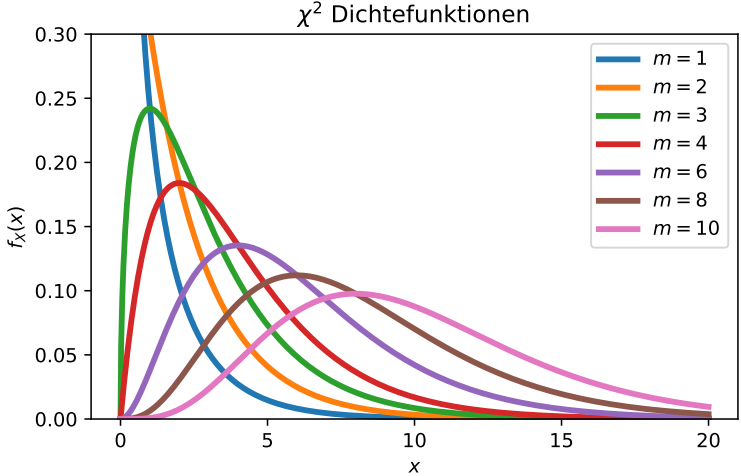
\includegraphics[width=\linewidth,keepaspectratio]{pictures/chi_squared_pdf.png} 
\end{figure}


\DEF{Gammafunktion}{$x\geq 0:\Gamma(x)=\int_0^{\infty}t^{x-1}e^{-t}dt$. Es gilt $\Gamma(n+1)=n!$ für $n\in\N_0$.}

\DEF{Studentsche t-Verteilung}{Sei $X$ stetige ZV. Falls für $x\in\R:$ $f_X(x)=\frac{\Gamma(\frac{m+1}{2})}{\sqrt{m\pi}\Gamma(\frac{m}{2})}(1+\frac{x^2}{m})^{-\frac{m+1}{2}}$ $\Rightarrow X\sim t_m$ $\Leftrightarrow X$ ist $t$-verteilt mit $m$ Freiheitsgraden.
\begin{enumerate}
    \item Entstehung: Sind $X\sim\mathcal{N}(0,1), Y\sim\chi_m^2$ unabhängig $\Rightarrow$ $\frac{X}{\sqrt{\frac{1}{m}Y}}\sim t_m$.
    \item Für $m=1$ erhält man eine Cauchy-Verteilung.
    \item Für $m\rightarrow\infty$ erhält man eine $\mathcal{N}(0,1)$-Verteilung.
    \item Ähnlich wie $\mathcal{N}(0,1)$ aber langschwänziger (long-tailed).
\end{enumerate}}
\begin{figure}[H]
 \centering
 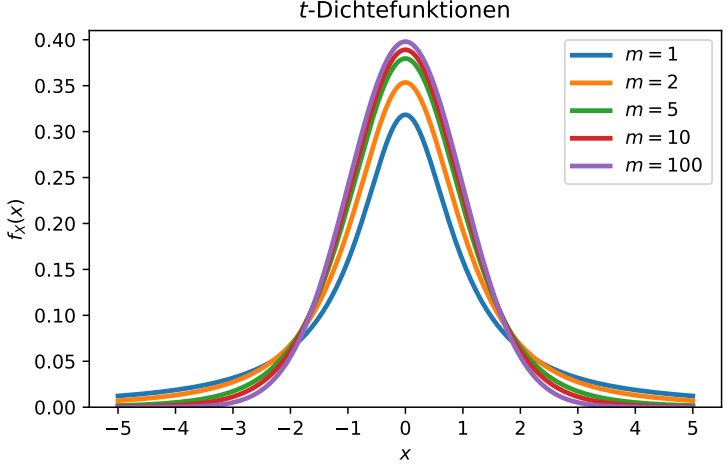
\includegraphics[width=\linewidth,keepaspectratio]{pictures/t_distribution_pdf.png} 
\end{figure}

\SA{7.20}{Seien $X_1,...X_n$ i.i.d. $\sim\mathcal{\mu,\sigma^2}$ und \begin{align*}
\overline{X}_n=\sum_{k=1}^n,\hspace{10px}S^2=\frac{1}{n-1}\sum_{k=1}^n(X_k-\overline{X}_n)^2.
\end{align*}

Es gelten folgende Aussagen:
\begin{align*}
    &1.\ \overline{X}_n\sim\mathcal{N}(\mu,\frac{1}{n}\sigma^2)\Leftrightarrow\frac{\overline{X}_n-\mu}{\frac{\sigma}{\sqrt{n}}}\sim\mathcal{N}(0,1),\\
    &2.\ \frac{n-1}{\sigma^2}S^2=\frac{1}{\sigma^2}\sum_{k=1}^n(X_k-\overline{X}_n)^2\sim\chi_{n-1}^2,\\
    &3.\ \overline{X}_n\ \text{und}\ S^2\ \text{sind unabhängig},\\
    &4.\ \frac{\overline{X}_n-\mu}{\frac{S}{\sqrt{n}}}=\frac{\frac{\overline{X}_n-\mu}{\sigma/\sqrt{n}}}{S/\sigma}=\frac{\frac{\overline{X}_n-\mu}{\sigma/\sqrt{n}}}{\sqrt{\frac{1}{n-1}\frac{n-1}{\sigma^2}S^2}}\sim t_{n-1}.
\end{align*}}

\mysection[LimeGreen]{Tests}

\mysubsection{Grundbegriffe}

\DEF{Grundprobem}{Entscheidung zwischen zwei konkurrierenden Modellklassen:
\begin{enumerate}
    \item die Hypothese (Nullhypothese, null hypothesis) $\Theta_0\subseteq\Theta$,
    \item die Alternative (Alternativhypothese, Gegenhypothese, alternative hypothesis) $\Theta_A\subseteq\Theta$.
\end{enumerate} wobei $\Theta_0\cap\Theta_A=\emptyset$.0}

\DEF{Hypothesen}{\begin{enumerate}
    \item Hypothese $H_0:\vartheta\in\Theta_0$,
    \item Alternative $H_A:\vartheta\in\Theta_A$.
\end{enumerate}

Wenn Alternative nicht explizit spezifiziert, dann $\Theta_A=\Theta_A^{\complement}=\Theta\setminus\Theta_0$.}

\DEF{Einfache Hypothesen/Alternativen}{$\Theta_0$ besteht aus einzelnem Wert $\Leftrightarrow$  $\Theta_0=\{\vartheta_0\}, |\Theta_0|=1$ $\Rightarrow$ $\Theta_0$ ist einfache Hypothese (dasselbe gilt analog für $\Theta_A$).}

\DEF{Zusammengesetzte Hypothgese/Alternative}{$\Theta_0$ nicht einfach $\Rightarrow$ $\Theta_0$ ist zusammengesetzte Hypothese (analog für $\Theta_A$).}

\DEF{Test}{Ein Paar $(T,K)$ wobei
\begin{enumerate}
    \item die Teststatistik $T=t(X_1,...,X_n)$ eine ZV mit $t:\R^n\rightarrow\R$ messbar,
    \item kritischer Bereich oder Verwerfungsbereich $K\subseteq\R$.
\end{enumerate}

Entscheidungsregel:
\begin{enumerate}
    \item $T(\omega)\in K\Rightarrow H_0$ wird verworfen,
    \item  $T(\omega)\not\in K\Rightarrow H_0$ wird angenommen.
\end{enumerate}}

\NOTE{8.3}{Die Entscheidung des Tests hängt von der Realisierung $\omega$ ab. Weil $T$ eine ZV ist, ist $\{T\in K\}=\{\omega\in\Omega|T(\omega)\in K\}$ eine (messbare) Teilmenge von $\Omega$, also ein Ereignis. Somit ist $\P_{\vartheta}[T\in K]$ über alle Modelle $\P_{\vartheta}$ hinweg bestimmbar.}

\DEF{Fehlerarten}{
\begin{enumerate}
    \item $H_0$ wird verworfen obschon richtig $\Leftrightarrow$ $\vartheta\in\Theta_0\land T\in K$. Sei $\vartheta\in\Theta_0$. Dann ist $\P_{\vartheta}[T\in K]$ die W'keit für einen Fehler 1. Art.
    \item $H_0$ wird angenommen obschon falsch $\Leftrightarrow$ $\vartheta\in H_A\land T\not\in K$. Sei $\vartheta\in\Theta_A$. Dann ist $\P_{\vartheta}[T\not\in K]=1-\P_{\vartheta}[T\in K]$ die W'keit für einen Fehler 2. Art.
\end{enumerate}}

\DEF{Zweistufiges Asymmetrisches Testvorgehen}{
\begin{enumerate}
    \item Wähle Signifikanzniveau $\alpha\in(0,1)$. Verlange $sup_{\vartheta\in\Theta_0}\P_{\vartheta}[T\in K]\leq\alpha$.
    \item Maximiere die Macht des Tests $\beta:\Theta_A\rightarrow[0,1],\vartheta\mapsto\beta(\vartheta)=\P_{\vartheta}[T\in K]$
\end{enumerate}

Seriöse Tests sollten immer die Negation der eigentlich gewünschten Aussage als Hypothese benutzen. Denn es ist schwieriger, die Hypothese anzunehmen als zu verwerfen. Es kann also passieren, dass die gleiche inhaltiche Frage zu unterschiedlichen Entscheidungen führt, wenn man bei ihrem Test Hypothese und Alternative vertauscht.}

\DEF{Randomisierter Test}{Wähle $\gamma\in[0,1]$ s.d. $\gamma\P_{\vartheta_0}[T>c]+(1-\gamma)\P_{\vartheta_0}[T>c+1]=\alpha$ und entscheide wie folgt: $T>0$ $\Rightarrow$ verwerfe $H_0$ mit W'keit $\gamma$. D.h.$H_0$ wird abgelehnt, falls \begin{enumerate}
    \item $T>c$, und
    \item eine unabhängige $\mathcal{U}(0,1)-$verteilte ZV einen Wert $\leq\gamma$ realisiert.
\end{enumerate}}

\mysubsection{Konstruktion von Tests}
Seien $X_1,...,X_n$ ZV, die entweder diskret, oder gemeinsam stetig unter $\P_{\vartheta_0}$ und $\P_{\vartheta_A}$ sind.

\DEF{Likelihood-Quotient}{Sei $\vartheta_0\in\Theta_0,\vartheta_A\in\Theta_A$ und $x_1,...,x_n\in\R$. Dann $R(x_1,...,x_n;\vartheta_0,\vartheta_A):=\frac{L(x_1,...,x_n;\vartheta_A)}{L(x_1,...,x_n;\vartheta_0)}$. Per Konvention gilt $L(x_1,...,x_n;\vartheta_0)=0$ $\Rightarrow$ $R(x_1,...,x_n;\vartheta_0,\vartheta_A)=\infty$.

Intuition: Desto grösser $R$ desto wahrscheinlicher ist $H_A$ gegenüber von $H_0$. Man verwirft $H_0$ also wenn $R$ gross wird.}

\DEF{Likelihood-Quotienten-Test}{Sei $c\geq 0$. Dann ist der Likelihood-Quotienten-Test mit Parameter $c$ ein Test $(T,K)$ mit $T=R(x_1,...,x_n;\vartheta_0,\vartheta_A)$ und $K=(c,\infty)$.}

\SA{8.9 Neyman-Pearson-Lemma}{Sei $\Theta_0=\{\vartheta_0\},\Theta_A=\{\vartheta_1\}$. Sei $(T,K)$ ein Likelihood-Quotienten-Test mit $c$ und $\alpha^*:=\P_{\vartheta_0}[T\in K]$. Ist $(T',K')$ ein anderer Test mit $\P_{\vartheta_0}[T'\in K']=:\alpha\leq\alpha^*$. Dann $\P_{\vartheta_A}[T'\in K']\leq\P_{\vartheta_A}[T\in K]$.

Intuition: Kleineres Signifikanzniveau führt zu kleinerer Macht bzw. grösserer W'keit für einen Fehler 2. Art.}

\DEF{Verallgemeinerter Likelihood-Quotient}{\begin{align*}
R(x_1,...,x_n)&=\frac{sup_{\vartheta\in\Theta_A}L(x_1,...,x_n;\vartheta)}{sup_{\vartheta\in\Theta_0}L(x_1,...,x_n;\vartheta)},\\
\tilde{R}(x_1,...,x_n)&=\frac{sup_{\vartheta\in\Theta_A\cup\Theta_0}L(x_1,...,x_n;\vartheta)}{sup_{\vartheta\in\Theta_0}L(x_1,...,x_n;\vartheta)}.
\end{align*}}

\EXAMPLE{8.11 Tea tasting lady}{Im Modell $\P_{\vartheta}$ sind $X_1,...,X_n$ i.i.d. $\sim Ber(\vartheta)$. Daraus folgt
\begin{align*}
    p_X(x_i;\vartheta)&=\vartheta^{x_i}(1-\vartheta)^{1-x_i}\\
\end{align*}
\begin{align*}
L(x_1,...,x_n;\vartheta)&=\prod_{i=1}^np_X(x_i;\vartheta)\\&=\vartheta^{\sum_{i=1}^nx_i}(1-\vartheta)^{n-\sum_{i=1}^nx_i}\\
\end{align*}
\begin{align*}
R(x_1,...,x_n;\vartheta_0,\vartheta_A)&=\frac{L(x_1,...,x_n;\vartheta_A}{L(x_1,...,x_n;\vartheta_0}\\
&=(\frac{\vartheta_A}{\vartheta_0})^{\sum_{i=1}^nx_i}(\frac{1-\vartheta_A}{1-\vartheta_0})^{n-\sum_{i=1}^nx_i}\\
&=(\frac{\vartheta_A(1-\vartheta_0)}{\vartheta_0(1-\vartheta_A)})^{\sum_{i=1}^nx_i}(\frac{1-\vartheta_A}{1-\vartheta_0})^n.\\
\end{align*}
Da wegen $\vartheta_0=\frac{1}{2}\land\vartheta_A>\frac{1}{2}\Rightarrow\vartheta_0 <\vartheta_A$. Gilt 
\begin{align*}
    \frac{\vartheta_A(1-\vartheta_0)}{\vartheta_0(1-\vartheta_A)}=\frac{\vartheta_A-\vartheta_A\vartheta_0}{\vartheta_0-\vartheta_A\vartheta_0}>1.
\end{align*}

Somit ist $R(x_1,...,x_n;\vartheta_0,\vartheta_A)$ gross $\Leftrightarrow$ $\sum_{i=1}^nx_i=S_n$ gross.

Wir wählen also als Teststatistik $T=S_n$ und als kritischen Bereich $K=(c,\infty)$.
}

\EXAMPLE{8.12}{Seien $X_1,...,X_n$ i.i.d. $\sim\mathcal{N}(\mu,\sigma^2)$ unter $\P_{\vartheta}$ mit $\sigma^2$ bekannt. Daraus folgt
\begin{align*}
        f_X(x_i;\vartheta)&=\frac{1}{\sigma\sqrt{2\pi}}exp(-\frac{(x_i-\vartheta)^2}{2\sigma^2})\\
\end{align*}
\begin{align*}
    L(x_1,...,x_n;\vartheta)&=\prod_{i=1}^nf_X(x_i;\vartheta)\\
    &=(2\pi\sigma^2)^{-\frac{n}{2}}exp(-\frac{1}{2\sigma^2}\sum_{i=1}^n(x_i-\vartheta)^2)\\
\end{align*}
\begin{align*}
R(x_1,...,x_n;\vartheta_0,\vartheta_A)&=\frac{L(x_1,...,x_n;\vartheta_A)}{L(x_1,...,x_n;\vartheta_0)}
\end{align*}
\begin{align*}
    &=exp(-\frac{1}{2\sigma^2}(\sum_{i=1}^n(x_i-\vartheta_A)^2-\sum_{i=1}^n(x_i-\vartheta_0)^2))\\
    &=C(\sigma,\vartheta_0,\vartheta_A)exp(\frac{1}{\sigma^2}(\vartheta_A-\vartheta_0)\sum_{i=1}^nx_i)\\
\end{align*}

wobei $C$ eine von $\sigma,\vartheta_0,\vartheta_A$ abhängige Konstante ist.

$R$ wird tendenziell gross, falls der Exponent $(\vartheta_A-\vartheta_0)\sum_{k=1}^nx_i$ gross ist. Hängt jedoch vom Vorzeichen $(\vartheta_A-\vartheta_0)$ ab.

Wir wählen als Teststatistik $T'=\sum_{i=1}X_i$.
\begin{enumerate}
    \item $(\vartheta_A-\vartheta_0)>0$, so wird der Exponent gross, wenn $T'$ gross wird. Wir wählen den kritischen Bereich von der Form $K_>'=(c_>',\infty)$, d.h. wir lehnen $H_0$ ab, wenn $T'$ gross ist.
    \item Ist $\vartheta_A-\vartheta_0<0$, so wird der Exponent gross für kleine $T'$ (d.h. negativ). Hier ist also der kritische Bereich von der Form $K_<'=(-\infty,c_<')$, d.h. wir lehnen $H_0$ ab, wenn $T'$ klein ist.
\end{enumerate}

In beiden Fällen mussen wir den kritischen Bereich noch so festlegen, dass der Test ein gewähltes Signifikanzniveau $\alpha$ einhält.
\begin{enumerate}
    \item Wir wollen $\P_{\vartheta_0}[T'\in K']\leq\alpha$. Dafür brauchen wir die Verteilung der Teststatistik $T'$ unter $\P_{\vartheta_0}$.
    \item In vorliegenden Fall ist das einfach. Unter jedem $\P_{\vartheta}$ sind $X_i$ i.i.d. $\sim\mathcal{N}(\mu,\sigma^2)$ $\Rightarrow$ $T'=\sum_{i=1}^nX_i\sim\mathcal{N}(n\vartheta,n\sigma^2)$ unter $\P_{\vartheta}$ $\Leftrightarrow$ $T=\frac{\overline{X}-\vartheta}{\frac{\sigma}{\sqrt{n}}}\sim\mathcal{N}(0,1)$ unter $\P_{\vartheta}$. Wir können also $T$ statt $T'$ als Teststatistik benutzen.
\end{enumerate}}

\DEF{Gauss-Test (Z-Test)}{Seien $X_1,...,X_n$ i.i.d. $\sim\mathcal{N}(\vartheta,\sigma^2)$ unter $\P_{\vartheta}$ mit $\sigma^2$ bekannt.
\begin{enumerate}
    \item Hypothese: $H_0:\vartheta=\vartheta_0$.
    \item Mögliche Alternativen: $H_A:$
    \begin{enumerate}
        \item $\vartheta >\vartheta_0$ (einseitig),
        \item $\vartheta <\vartheta_0$ (einseitig),
        \item $\vartheta\not =\vartheta_0$ (zweiseitig).
    \end{enumerate}
\end{enumerate}

Sei wie in Beispiel 8.12 $T=\frac{\overline{X}-\vartheta}{\frac{\sigma}{\sqrt{n}}}\sim\mathcal{N}(0,1)$ unter $\P_{\vartheta_0}$.

$K$ ist von der Form:
\begin{enumerate}
    \item $(c_>,\infty)$ bzw. $(-\infty,c_<)$ für einseitige Tests gegen die Alternative $H_A:\vartheta >\vartheta_0$ bzw. $H_A:\vartheta < \vartheta_0$, oder
    \item $(-\infty,-c_{\not =})\cup(c_{\not=},\infty)$ für den zweiseitigen Fall. $H_0$ verwirft man hier zugunsten der Alternative $H_A:\vartheta\not=\vartheta_0$ falls  $|T|>c_{\not=}$.
\end{enumerate}

Signifikanzniveau für $\mathcal{N}(0,1)$:
\begin{enumerate}
    \item $\vartheta >\vartheta_0$: $\alpha=\P_{\vartheta_0}[T\in K_{>}]=\P_{\vartheta_0}[T>c_>]=1-\P_{\vartheta_0}[T\leq c_>]=1-\Phi(c_>)$ $\Rightarrow$ $c_>=\Phi^{-1}(1-\alpha)=:z_{1-\alpha}$ ist das $(1-\alpha)-$Quantil der $\mathcal{N}(0,1)-$Verteilung. Für $\vartheta >\vartheta_0$ verwirft man also $H_0$, falls $\overline{X}_n >\vartheta_0+z_{1-\alpha}\frac{\sigma}{\sqrt{n}}$.
    \item $\vartheta <\vartheta_0$: $c_<=z_{\alpha}=-z_{1-\alpha}$. Es gilt $\alpha=\P_{\vartheta_0}[T<c_<]=\P_{\vartheta_0}[T>-c_<]$ für $-c_<=z_{1-\alpha}$.
    \item $\vartheta\not=\vartheta_0$: $c_{\not=}=z_{1-\frac{\alpha}{2}}$. Es gilt $\alpha=\P_{\vartheta_0}[T\in K_{\not=}]=\P_{\vartheta_0}[T<-c_{\not=}]+\P_{\vartheta_0}[T>c_{\not=}]=\Phi(-c_{\not=})+1-\Phi(c_{\not=})=2(1-\Phi(c_{\not=})$.
\end{enumerate}


}

\mysection[WildStrawberry]{Beispiele}

\mysubsection{Würfel}
1) Mindestens eine Sechs bei 4 Würfen mit einem Würfel: $1-(\frac{5}{6})^4 = 51.78\%$.

2) Mindestens ein Sechserpasch beim 24-maligen Werfen von zwei Würfeln: $1-(\frac{35}{36})^{24} = 49.14\%$.

3) Genau eine Sechs beim Werfen von 12 Würfeln: ${12\choose 1}(\frac{5}{6})^{11}(\frac{1}{6})=26.92\%$.

4) Genau zwei Sechsen beim Werfen von 12 Würfeln: ${12\choose 2}(\frac{5}{6})^{10}(\frac{1}{6})^2=29.61\%$

5) Mindestens zwei Sechsen beim Werfen von 12 Würfeln: $1 - ((\frac{5}{6})^{12} + {12\choose 1}(\frac{5}{6})^{11}(\frac{1}{6}))=61.87\%$

\mysubsection{Zufallsvariable}
1) Wirft man eine Münze zweimal, so ist $\Omega=\{KK,KZ,ZK,ZZ\}$ und $\mathcal{F}=\mathcal{P}(\Omega)$. Eine mögliche ZV $X_1$ ist die Gesamtanzahl geworfener Köpfe: $X = \begin{cases}
    0 & \text{if } \omega = ZZ, \\
    1 & \text{if } \omega = ZK \lor \omega = KZ, \\
    2 & \text{if } \omega = KK.
  \end{cases}$

2) Man wirft eine Münze solange bis man Kopf erhält $\Omega=\{K,ZK,ZZK,...\}$. Dann ist die Gesamtzahl der Würfe $X$ eine ZV, welche auch Wartezeit bis zum ersten Erfolg heisst. $X = \begin{cases}
    1 & \text{if } \omega = K, \\
    2 & \text{if } \omega = ZK, \\
    3 & \text{if } \omega = ZZK, \\
    \hdots &
  \end{cases}$


\mysubsection{Verteilungsfunktion}
1) Sei $A\in\mathcal{F}$ und $X=1_A$ die Indikatorfunktion. Dann ist die Verteilungsfunktion gegeben durch

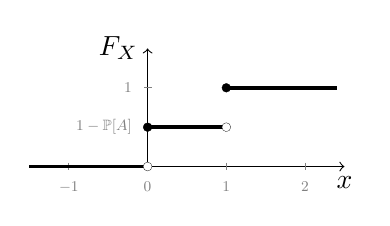
\begin{tikzpicture}
    \draw[->] (-1.5, 0) -- (2.5, 0) node[below] {$x$};
    \draw[->] (0, 0) -- (0, 1.5) node[left]{$F_X$};
    \foreach \x in {-1, ..., 2} {
        \draw [gray] (\x, 0.05) -- ++(0, -.1) ++(0, -.15) node [below, outer sep=0pt, inner sep=0pt, scale=0.6] {\small\(\x\)};}
    \foreach \y in {1} {
        \draw [gray] (0.05, \y) -- ++(-.1, 0) ++(-.15, 0) node [left, outer sep=0pt, inner sep=0pt, scale=0.6] {\small\(\y\)};}
    \draw [gray] (0.05, 0.5) -- ++(-.1, 0) ++(-.15, 0) node [left, outer sep=0pt, inner sep=0pt, scale=0.6] {\small\(1-\mathbb{P}[A]\)};
    \draw[draw=black,line width=1.3pt] (-1.5,0) -- (0,0);
    \draw[draw=black,line width=1.3pt] (0,0.5) -- (1,0.5);
    \draw[draw=black,line width=1.3pt] (1,1) -- (2.4,1);
    \filldraw[draw=black,line width=0.1pt,fill=white] (0,0) circle[radius=1.6pt];
    \filldraw[draw=black,line width=0.1pt,fill=black] (0,0.5) circle[radius=1.6pt];
    \filldraw[draw=black,line width=0.1pt,fill=white] (1,0.5) circle[radius=1.6pt];
    \filldraw[draw=black,line width=0.1pt,fill=black] (1,1) circle[radius=1.6pt];
\end{tikzpicture}

$F_X(x) = \begin{cases}
    0 & \text{if } x<0, \\
    1-\P(A) & \text{if } 0\leq x<1, \\
    1 & \text{if } x\geq 1.
\end{cases}$

2) Sei $X$ eine ZV mit cfd $F_X$. Sei $Y=exp(X)=e^X$. Dann ist $F_Y(x)=\P[Y\leq x]=\P[e^X\leq x]=\P[log(e^X)\leq log(x)]=\P[X\leq log(x)]=F_X(log(x))$. Weil $e^X>0$ $\forall x\in\R \Rightarrow \P[e^X\leq x]=0$ $\forall x\leq 0$. Somit erhalten wir
 
$F_Y(x) = \begin{cases}
    0 & \text{if } x\leq 0, \\
    F_X(log(x)) & \text{if } x>0.
\end{cases}$
\mysection[Aquamarine]{\centering Weiteres}
\mysubsection{Rechenregeln für Summen}
\begin{enumerate}
    \item $\sum_{i=L}^Ux_i=\sum_{i=L}^{I-1}x_i+\sum_{i=I}^Ux_i$
    \item $\sum_{i=L}^Ucx_i=c\sum_{i=L}^Ux_i$
    \item $\sum_{i=L}^Ux_i\pm\sum_{i=L}^Uy_i=\sum_{i=L}^U(x_i\pm y_i)$
    \item $\sum_{i=L_1}^{U_1}x_{i_1}\cdot ... \cdot \sum_{i=L_n}^{U_n}x_{i_n}=\sum_{i=L_1}^{U_1}\cdot ... \cdot \sum_{i=L_n}^{U_n}(x_{i_1}\cdot ...\cdot x_{i_n})$
    \item $\sum_{i=L_1}^{U_1}\sum_{j=L_2}^{U_2}x_{i,j}=\sum_{j=L_2}^{U_2}\sum_{i=L_1}^{U_1}x_{i,j}$
\end{enumerate}

\mysubsection{Summenformeln}
\begin{enumerate}
    \item $\sum_{i=1}^{n} i = 1 + 2 + 3 + ... + n = \frac{n(n+1)}{2} = \frac{1}{2}n^2 + \frac{1}{2}n$
    \item $\sum_{i=1}^{n} i^2 = 1^2 + 2^2 + 3^2 + ... + n^2 = \frac{n(n+1)(2n + 1)}{6} = \frac{1}{3}n^3 + \frac{1}{2}n^2 + \frac{1}{6}n$
    \item $\sum_{i=1}^{n} i^3 = 1^3 + 2^3 + 3^3 + ... + n^3 = \frac{n^2(n+1)^2}{4} = \frac{1}{4}n^4 + \frac{1}{2}n^3 + \frac{1}{4}n^2$
    \item $\sum_{k=0}^{n} aq^k = aq^0 + aq^1 + aq^2 + ... + aq^n = \frac{a(q^{n+1}-1)}{q-1}=\frac{a(1-q^{n+1})}{1-q}$
    \item $(j+1)^2 - j^2 = 2j + 1$
    \item $C_1 \cdot n^{k+1} \leq \sum_{i=1}^{n} i^k \leq C_2 \cdot n^{k+1}$ where $C_1 = \frac{1}{2^{k+1}}$ and $C_2 = 1$ are two constants independent of $n$. Hence, when n is large, $\sum_{i=1}^n i^k$ behaves "almost like $n^{k+1}$" up to a constant factor. In other words $\sum_{i=1}^n i^k = \theta (n^{k+1})$.
\end{enumerate}


\mysubsection{Grenzwerte}
\DEF{Asymptotisches Wachstumsverhalten}{$lim_{n\rightarrow\infty}:1<\log(\log(n))<\log(n)<\sqrt{n}<n<n\log(n)<n^2<2^n<n!<n^n$.}

\DEF{Wichtige Grenzwerte}{\begin{enumerate}
    \item $lim_{n\rightarrow\infty}(1 + \frac{1}{n})=1$.
    \item $lim_{n\rightarrow\infty}(1 + \frac{1}{n})^b=1^b=1$\hspace*{\fill}$ \forall b\in\mathbb{Z}$.
    \item $lim_{n\rightarrow\infty}n^aq^n=0$\hspace*{\fill}$ \forall a\in\mathbb{Z},0\leq q < 1$.
    \item $lim_{n\rightarrow\infty}(\frac{1}{1+\varepsilon})^n=0$\hspace*{\fill}$ \forall \varepsilon>0$.
    \item $lim_{n\rightarrow\infty}\sqrt[n]{a}=1$\hspace*{\fill}$ \forall a\in\mathbb{R},a>0$.
    \item $lim_{n\rightarrow\infty}(1+\frac{z}{n})^n=exp(z)$.
    \item $lim_{x\rightarrow 0^+}ln(x)=-\infty$.
    \item $lim_{x\rightarrow 0^+}x^a=0$\hspace*{\fill}$a>0$.
    \item $lim_{x\rightarrow 0}\frac{sin(x)}{x}=1$\hspace*{\fill}$ x\in D=\mathbb{R}\setminus\{0\}$.
    \item $lim_{x\rightarrow 0}\frac{cos(x)-1}{x}=0$.
\end{enumerate}}


\mysubsection{Reihen}
\DEF{Definitionen per Potenzreihe}{
\begin{enumerate}
    \item $exp(x)=\sum_{n=0}^{\infty}\frac{x^n}{n!}$\hspace*{\fill} $\rho=\infty$.
    \item $sin(x)=\sum_{n=0}^{\infty}(-1)^n\frac{x^{2n+1}}{(2n+1)!}$\hspace*{\fill} $\rho=\infty$.
    \item $cos(x)=\sum_{n=0}^{\infty}(-1)^{n}\frac{x^{2n}}{(2n)!}$\hspace*{\fill} $\rho=\infty$.
    \item $ln(x+1)=\sum_{n=0}^{\infty}(-1)^{n+1}\frac{x^n}{n}$\hspace*{\fill} $\rho=1$.
\end{enumerate}}

\DEF{Wichtige Reihen}{\begin{enumerate}
    \item $\sum_{n=0}^{\infty}\frac{1}{n}$ divergiert.
    \item $\sum_{n=0}^{\infty}\frac{1}{n^p}$ konvergiert $\forall p>1$.
    \item $\sum_{n=0}^{\infty}\frac{(-1)^n}{n}$ konvergiert, aber nicht absolut.
    \item $\sum_{n=0}^{\infty}\frac{1}{n^2}=\frac{\pi^2}{6}$.
    \item $\sum_{n=0}^{\infty}\frac{1}{n(n+1)}=1$.
    \item $\sum_{n=0}^{\infty}aq^n=\frac{a}{1-q}$\hspace*{\fill}$q\in\mathbb{C},|q|<0,a\in\mathbb{R}$.
\end{enumerate}}



\mysubsection{Uneigentliche Integrale}
\begin{enumerate}
    \item $\int_0^{\infty}e^{-x}dx=1$
    \item $\int_1^{\infty}\frac{1}{x^a}dx=\begin{cases}
    divergiert & \alpha\leq 1,\\
    \frac{1}{\alpha-1} & \alpha > 1.
    \end{cases}$
    \item $\int_0^1\frac{1}{x^a}dx=\begin{cases}
    divergiert & \alpha \geq 1,\\
    \frac{1}{1-\alpha} & \alpha < 1.
    \end{cases}$
\end{enumerate}


\mysubsection{Ableitungen}
\begin{center}
  % the c>{\centering\arraybackslash}X is a workaround to have a column fill up all space and still be centered
  \begin{tabularx}{\linewidth}{c>{\centering\arraybackslash}Xc}
  \toprule
  $\mathbf{F(x)}$ & $\mathbf{f(x)}$ & $\mathbf{f'(x)}$ \\
  \midrule
  $x$ & $c$ & $0$ \\[3px]
  $\frac{x^{c+1}}{c+1}$ & $x^c$ & $c \cdot x^{c-1}$ \\[3px]
  $\ln |x|$ & $\frac{1}{x}$ & $-\frac{1}{x^2}$ \\[3px]
  $\frac{x^{-c+1}}{-c+1}$ & $\frac{1}{x^c}$ & $\frac{-c}{x^{c+1}}$ \\[3px]
  $\frac{2}{3}x^{3/2}$ & $\sqrt{x}$ & $\frac{1}{2\sqrt{x}}$\\[3px]
  $\frac{1}{c \ln(a)}a^{cx}$ & $a^{cx}$ & $ca^{cx} \ln(a)$ \\[3px]
  $-\cos(x)$ & $\sin(x)$ & $\cos(x)$ \\[3px]
  $\sin(x)$ & $\cos(x)$ & $-\sin(x)$ \\[3px]
  $\frac{1}{2}(x-\frac{1}{2}\sin(2x))$ & $\sin^2(x)$ & $2 \sin(x)\cos(x)$ \\[3px]
  $\frac{1}{2}(x + \frac{1}{2}\sin(2x))$ & $\cos^2(x)$ & $-2\sin(x)\cos(x)$ \\[3px]
  $-\ln|\cos(x)|$ & $\tan{x}$ & $1+\tan^2(x)=\frac{1}{cos^2(x)}$\\[3px]
  $\ln | \sin(x)|$ & $\cot(x)$ & $\frac{-1}{\sin^2(x)}$ \\[3px]
  $\cosh(x)$ & $\sinh(x)$ & $\cosh(x)$ \\[3px]
  $\ln|\cosh(x)|$ & $\tanh(x)$ & $\frac{1}{\cosh^2(x)}$ \\[3px]
  $\frac{1}{c} \cdot e^{cx}$ & $e^{cx}$ & $c \cdot e^{cx}$ \\[3px]
  $x(\ln |x| - 1)$ & $\ln |x|$ & $\frac{1}{x}$ \\[3px]
  $\frac{1}{2}(\ln(x))^2$ & $\frac{\ln(x)}{x}$ & $\frac{1 - \ln(x)}{x^2}$ \\[3px]
  $\frac{x}{\ln(a)} (\ln|x| -1)$ & $\log_a |x|$ & $\frac{1}{\ln(a)x}$ \\[3px]
  $ $ & $\arcsin(x)$ & $\frac{1}{\sqrt{1-x^2}}$ \\[3px]
  $ $ & $\arccos(x)$ & $\frac{-1}{\sqrt{1-x^2}}$ \\[3px]
  $ $ & $\arctan(x)$ & $\frac{1}{1+x^2}$ \\[3px]
  $ $ & $\text{arccot}(x)$ & $\frac{-1}{1+x^2}$ \\[3px]
  $ $ & $\text{arsinh}(x)$ & $\frac{1}{\sqrt{x^2+1}}$ \\[3px]
  $ $ & $\text{arcosh}(x)$ & $\frac{-1}{\sqrt{x^2-1}}$ \\[3px]
  $ $ & $\text{artanh}(x)$ & $\frac{1}{1-x^2}$ \\[3px]
  \bottomrule
  \end{tabularx}
\end{center}


\mysubsection{Algebraische Gesetze}
\DEF{Quadratische Gleichungen Lösen}{$f(x)=ax^2+bx+c=0 \Rightarrow x=\frac{-b\pm\sqrt{D}}{2a}=\frac{-b\pm\sqrt{b^2-4ac}}{2a}$. \begin{itemize}
    \item $D=0\Rightarrow f$ hat eine Nullstelle
    \item $D>0\Rightarrow f$ hat zwei Nullstellen
    \item $D<0\Rightarrow f$ hat keine Nullstellen.
\end{itemize}}

\DEF{Faktorisierung spezieller Polynome}{
\begin{enumerate}
    \item $x^2-y^2=(x+y)(x-y)$
    \item $x^3+y^3=(x+y)(x^2-xy+y^2)$
    \item $x^3-y^3=(x-y)(x^2+xy+y^2)$
\end{enumerate}}

\DEF{Binomische Formel}{Für $n\in\mathbb{N}: (x+y)^n=\sum_{k=0}^n{n\choose k}x^{n-k}y^k$ wobei ${n\choose k}$ der Binomialkoeffizient "n tief k" ist: ${n\choose k}=\frac{n!}{k!(n-k)!}=\frac{n\cdot (n-1) \cdot (n-2) \cdot ... \cdot (n-k+1)}{k\cdot (k-1) \cdot ... \cdot 3 \cdot 2 \cdot 1}={n\choose n-k}$.

\begin{tabular}{>{$n=$}l<{\hspace{25pt}}*{13}{c@{\hspace{2pt}}}}
0 &&&&&&&1&&&&&&\\
1 &&&&&&1&&1&&&&&\\
2 &&&&&1&&2&&1&&&&\\
3 &&&&1&&3&&3&&1&&&\\
4 &&&1&&4&&6&&4&&1&&\\
5 &&1&&5&&10&&10&&5&&1&\\
6 &1&&6&&15&&20&&15&&6&&1
\end{tabular}}


\DEF{Potenzieren}{\begin{enumerate}
    \item $a^m\cdot a^n=a^{m+n}$
    \item $\frac{a^m}{a^n}=a^{m-n}=\frac{1}{a^{n-m}}$
    \item $(a^m)^n=a^{mn}=(a^n)^m$
    \item $a^n\cdot b^n=(ab)^n$
    \item $\frac{a^n}{b^n}=(\frac{a}{b})^n, b\not =0$
    \item $a^{-n}=\frac{1}{a^n} \Leftrightarrow a^{n}=\frac{1}{a^{-n}}$
\end{enumerate}}

\DEF{Radizieren}{
\begin{enumerate}
    \item $\sqrt[n]{a}\cdot\sqrt[n]{b}=\sqrt[n]{ab}$
    \item $\frac{\sqrt[n]{a}}{\sqrt[n]{b}}=\sqrt[n]{\frac{a}{b}},b\not=0$
    \item $\sqrt[n]{\sqrt[m]{a}}=\sqrt[n\cdot m]{a}$
    \item $a^{\frac{n}{m}}=\sqrt[m]{a^n}=\frac{1}{a^{-\frac{n}{m}}}$
\end{enumerate}}

\DEF{Logarithmieren}{
\begin{enumerate}
    \item $log_ac=\frac{ln(c)}{ln(a)}$
    \item $log_a(u\cdot v)=log_au+log_av$
    \item $log_a(\frac{u}{v})=log_au-log_av\Leftrightarrow log_a(\frac{1}{v})=-log_a(v)$
    \item $log_a(b^n)=n\cdot log_ab$
    \item $y=q^x\Rightarrow x=\frac{ln(y)}{ln(q)}=log_qy\Rightarrow q^{log_qy}=y$
    \item $u^{log_av} = v^{log_au}$
\end{enumerate}}

\DEF{Weitere nützliche Eigenschaften}{
\begin{enumerate}
    \item $\frac{u}{v}\geq\frac{w}{x} \Leftrightarrow \frac{v}{u}\leq \frac{x}{w}\ \forall u,v,w,x\in\mathbb{R},u\not=0,v\not=0,w\not=0,x\not=0$.
    \item $1-x\leq e^{-x}\Leftrightarrow 1+x\leq e^x\ \forall x\in\mathbb{R}$
    \item Sei $x>0,a\in\mathbb{R}$. Dann $x^a=e^{{ln(x)}^a}=e^{ln(x)\cdot a}=exp(a\cdot ln(x))$.
\end{enumerate}}

\mysubsection{Algebraische Methoden}
\DEF{Umkehrfunktion}{Verwenden von $log$ und $e$ für die Vereinfachung von Gleichungen mit Potenzen/Exponenten, z.B. $lim_{n\rightarrow\infty}\frac{n^{\frac{2n+3}{n+1}}}{n^2}=lim_{n\rightarrow\infty}n^{\frac{2n+3}{n+1}-2}=lim_{n\rightarrow\infty}n^{\frac{1}{n+1}}=lim_{n\rightarrow\infty}e^{ln(n^{\frac{1}{n+1}})}=lim_{n\rightarrow\infty}e^{\frac{ln(n)}{n+1}}=e^0=1$.}

\DEF{Rationalisieren des Nenners}{Elimination der Wurzel im Nenner, z.B. $\frac{1}{\sqrt{2}}=\frac{1}{\sqrt{2}}\cdot\frac{\sqrt{2}}{\sqrt{2}}=\frac{\sqrt{2}}{2}$ oder $\frac{2}{\sqrt[4]{3x^2}}=\frac{2}{\sqrt[4]{3x^2}}\cdot\frac{\sqrt[4]{3^3x^2}}{\sqrt[4]{3^3x^2}}=\frac{2\sqrt[4]{27x^2}}{\sqrt[4]{3^4x^4}}=\frac{2\sqrt[4]{27x^2}}{3|x|}$.

Wenn der Nenner aus zwei Termen besteht, muss man mit dem dem Konjugat des Nenners multiplizieren, z.B. $\frac{1}{4-\sqrt{x}}=\frac{1}{4-\sqrt{x}}\cdot\frac{4+\sqrt{x}}{4+\sqrt{x}}=\frac{4+\sqrt{x}}{4^2+4\sqrt{x}-4\sqrt{x}+x}=\frac{4+\sqrt{x}}{16-x}$.}

\DEF{Rationalisieren des Zählers}{Selbes Prinzip wie Oben, einfach angewandt auf den Zähler.}

\DEF{Linearfaktorzerlegung}{Ein Polynom von der Polynomform in die Produktform bringen. Die Nullstellen des Polynoms können von der Produktform direkt abgelesen werden. 
\begin{enumerate}
    \item Vorfaktor ausklammern
    \item Nullstellen berechnen
    \item Linearfaktoren aufstellen
    \item in Produktform bringen
\end{enumerate}
Beispiel: 
$f(x)=2x^2+3x+1 \Leftrightarrow f(x)=2(x^2+\frac{3}{2}x+\frac{1}{2})$. 

$x_1,x_2=\frac{-1.5\pm\sqrt{1.5^2-4\cdot 1 \cdot 0.5}}{2\cdot 1} \Rightarrow x_1=-\frac{1}{2},x_2=-1$.

$f(x)=2(x-x1)(x-x2)=2(x+\frac{1}{2})(x+1)$.

Beispiel:
$f(x)=x^3-6x^2+5x \Leftrightarrow f(x)=x(x^2-6x+5) \Rightarrow x_1=0$.

$x_2,x_3=\frac{6\pm\sqrt{6^2-4\cdot 1 \cdot 5}}{2\cdot 1} \Rightarrow x_2=5,x_3=1$.

$f(x)=(x-x1)(x-x2)(x-x_3)=x(x-5)(x-1)$.

Merke:

Für Polynome 3. Grades bei welchen wir nicht einfach $x$ ausklammern können, verwenden wir Polynomdivision durch einen Linearfaktor.}

\DEF{Polynomdivision}{Ähnlich wie schriftliche Division einfach für Polynome. Anleitung: \begin{enumerate}
    \item Fehlende Potenzen mit einem $0$-Koeffizienten auffüllen.
    \item Rechter Pivot durch linker Pivot teilen.
    \item Ergebnis mit Divisor multiplizieren.
    \item Minus rechnen.
\end{enumerate}

Beispiel ohne Rest:

\hspace{6px}$(x^2-3x+2):(x-1)=x-2$

\underline{$-(x^2-x)$}

\hspace{20px}$-2x+2$

\hspace{11px}\underline{$-(-2x+2)$}

\hspace{45px}$0\Rightarrow$ kein Rest, fertig.

Beispiel mit Rest:

\hspace{6px}$(5x^3+0x^2-7x+9):(x-2)=5x^2+10x+13+\frac{35}{x-2}$

\underline{$-(5x^3-10x^2)$}

\hspace{32px}$10x^2-7x$

\hspace{23px}\underline{$-(10x^2-20x)$}

\hspace{59px}$13x+9$

\hspace{50px}\underline{$-(13x-26)$}

\hspace{82px}$35\Rightarrow$ mit Rest $\Rightarrow$ durch Divisor teilen und oben addieren.
}

\DEF{Partialbruchzerlegung}{Ziel ist eine rationale Funktion als Summe von Brüchen darzustellen, wobei der Grad aller Nenner $\leq$ 2. Sei $R(x)=\frac{P(x)}{Q(x)}$ eine rationale Funktion. Seien $\gamma_1,...,\gamma_k$ die reellen Nullstellen und $\alpha_1\pm i\beta_1,...,\alpha_l\pm i\beta_l$ die komplexen Nullstellen. Sei $n_i$ die Vielfachheit von $\gamma_i$. Sei $m_j$ die Vielfachheit von $\alpha_j\pm i\beta_j$.

Anleitung:
\begin{enumerate}
    \item Reduktion auf den Fall $deg(P) < deg(Q)$. Falls dies bereits gilt $\rightarrow$ (2). Falls nicht berechne mittels Polynomdivision $S(x),\hat{P}(x):P(x)=S(x)Q(x)+\hat{P}(x)\Leftrightarrow\frac{P(x)}{Q(x)}=S(x)+\frac{\hat{P}(x)}{Q(x)},deg(\hat{P})<deg(Q)$.
    \item Linearfaktorzerlegung von $Q$. Also $Q(x)=\prod_{j=1}^l((x-\alpha_j)^2+\beta^2_j)^{m_j}\prod_{i=1}^k(x-\gamma_i)^{n_i}$.
    \item Partialbrüche anhand Linearfaktoren aufstellen. \begin{itemize}
        \item Einfache Nullstellen (Vielfachheit 1): Sei $C_i\in\mathbb{R}\ \forall i\in[k]$. Dann $\frac{P(x)}{Q(x)}=\sum_{i=1}^k \frac{C_{i}}{(x-\gamma_i)}$.
        \item Allgemeine Nullstellen:  Sei $C_{ij}\in\mathbb{R}\ \forall i\in[k],j\in[n_i]$. Dann $\frac{P(x)}{Q(x)}=\sum_{i=1}^k\sum_{j=1}^{n_i} \frac{C_{ij}}{(x-\gamma_i)^j}$.
        \item Allgemeine Nullstellen (auch Komplexe): Sei $C_{ij}\in\mathbb{R}\ \forall i\in[k],j\in[n_i]$. Sei $A_{ij},B_{ij}\in\mathbb{R}\ \forall i\in[l],j\in[m_i]$. Dann $\frac{P(x)}{Q(x)}=\sum_{i=1}^l\sum_{j=1}^{m_i}\frac{A_{ij}+B_{ij}x}{((x-\alpha_i)^2+\beta^2_i)^j}+\sum_{i=1}^k\sum_{j=1}^{n_i}\frac{C_{ij}}{(x-\gamma_i)^j}$.
    \end{itemize}
    \item Mithilfe von Koeffizienten-Vergleich ein GLS aufstellen und so $C_{ij},A_{ij},B_{ij}$ berechnen.
\end{enumerate}}


\end{flushleft}
\end{multicols}
\end{document}
